\documentclass[letterpaper]{article}
\usepackage{lindrew}
\usepackage{titling}
\usepackage{float}
\usepackage{booktabs}
\usepackage{subcaption}

\hypersetup{pdftitle={GitHub Network Analysis}, pdfauthor={Farhan Sadeek}}
\begin{document}
\title{\textbf{Analyzing the GitHub Social Network} \\ \Large A Comprehensive Study of the MUSAE Developer Graph}
\author{Farhan Sadeek}
\date{\today}

\maketitle
\tableofcontents
\newpage

%% ============================================================
\section{Introduction}
%% ============================================================

Who are the most influential developers on GitHub, and what holds their social network together? To answer these questions, we analyze the GitHub mutual-follower network from the MUSAE (Multi-Scale Attributed Node Embedding) project~\cite{rozemberczki2021musae}---a rich dataset of 37,700 developers connected by 289,003 mutual-follower relationships, collected via the GitHub API in June 2019. Every developer in the dataset starred at least ten repositories, and each carries a binary label: \emph{Web Developer} (class~0) or \emph{Machine Learning Engineer} (class~1), based on their self-reported job title.

We follow the analytical framework of Kolaczyk and Csardi~\cite{kolaczyk2020sand}, working through seven stages: exploratory visualization, degree and centrality analysis, community detection, spectral decomposition, random graph model comparisons, statistical network modeling (block models, dyadic regression, latent embeddings), and link prediction. Each stage builds on the last, and together they reveal a network that is sparse yet tightly connected, dominated by a handful of super-hubs, and shaped by strong professional homophily.

\subsection{Prior Work}

The MUSAE dataset comes from the Stanford Network Analysis Project (SNAP). Rozemberczki et al.~\cite{rozemberczki2021musae} used it to develop a multi-scale node embedding method that outperformed DeepWalk, Node2Vec, and GraphSAGE on node classification tasks. But their focus was embedding quality, not the network's structure. That leaves an open question: what does the GitHub follower network actually look like, and what forces shape it? That is what we set out to explore.

\subsection{The MUSAE Algorithm}

The MUSAE project was initiated to solve a critical limitation in existing graph representation learning: the inability to effectively integrate node-level attributes with topological structure across varying scales. Traditional methods like DeepWalk~\cite{perozzi2014deepwalk} and Node2Vec~\cite{grover2016node2vec} focus on path-based proximity and often overlook the features associated with developers (e.g., location, employer, starred repositories).

MUSAE employs a Skip-gram style approach but reorients the objective to capture the distribution of attributes within a node's neighborhood rather than just the node's identity. The framework defines two primary strategies:

\begin{itemize}
  \item \textbf{Pooled Attributed Embedding (AE)}: Observations from neighborhoods of different sizes are averaged or pooled, creating a single, aggregated feature representation for each node.
  \item \textbf{Multi-Scale Attributed Node Embedding (MUSAE)}: Observations are encoded distinctly at each scale (proximity $r$). This captures the nuance that a developer's immediate neighbors (close collaborators) might have different attribute profiles than their distant neighbors (friends-of-friends).
\end{itemize}

Mathematically, the algorithm implicitly factorizes matrices of node-feature Pointwise Mutual Information (PMI). By doing so, it ensures that nodes with similar local attribute distributions are positioned close together in the latent embedding space, even if they are not directly connected. A major advantage is computational efficiency: MUSAE utilizes approximated matrix powers instead of exhaustive random walks, significantly reducing the time and memory required for training.

\begin{table}[H]
  \centering
  \begin{tabular}{llll}
    \toprule
    \textbf{Algorithm} & \textbf{Mechanism} & \textbf{Scalability} & \textbf{Attribute Awareness} \\
    \midrule
    DeepWalk   & Random walks          & Medium & Low  \\
    Node2Vec   & Biased walks          & Medium & Low  \\
    Walklets   & Multi-scale topology  & Low    & Low  \\
    GCN        & Spectral convolution  & Medium & High \\
    MUSAE      & PMI factorization     & High   & High \\
    \bottomrule
  \end{tabular}
  \caption{Comparison of graph embedding algorithms. MUSAE uniquely combines high scalability with high attribute awareness through PMI factorization rather than random walks.}
  \label{tab:embedding_algorithms}
\end{table}

The MUSAE approach has been shown to outperform classic models on node classification tasks while remaining computationally feasible for graphs exceeding 100,000 nodes~\cite{rozemberczki2021musae}. This efficiency is crucial for industrial applications where network structures evolve rapidly and embeddings must be updated frequently.

\subsection{Motivation}

GitHub is where much of the world's open-source software lives. Millions of developers use it daily, and for many, their GitHub profile doubles as a professional portfolio---recruiters in Software Engineering and Data Science routinely ask to see it. But GitHub is not just a code-hosting platform; it is also a social network. Developers follow each other, forming a web of connections that reflects professional interests, admiration, and collaboration.

Understanding the structure of this social web matters. It can reveal who the most influential developers are, how knowledge communities form, and whether professional specialization---Web Development vs.\ Machine Learning---shapes who connects with whom. These are the questions we explore in this article.

\subsection{Limitations}

Before diving in, a few caveats worth keeping in mind:
\begin{itemize}
  \item \textbf{Temporal snapshot}: The data was collected in June 2019, predating the massive surge in AI/ML popularity driven by large language models. The relative proportions of Web vs.\ ML developers---and their interconnections---have likely shifted substantially since then.
  \item \textbf{Binary classification}: Labeling developers as either ``Web Developer'' or ``ML Engineer'' is a coarse simplification. Many developers hold hybrid roles (e.g., MLOps, full-stack data science), and the labeling methodology is not described in detail.
  \item \textbf{Single relationship type}: Mutual-follower relationships capture only one dimension of developer interaction. Contributions to shared repositories, issue discussions, code reviews, and star activity are not represented in the edge set.
  \item \textbf{Selection bias}: Only developers who starred at least ten repositories are included, which skews the sample toward more active and engaged users.
\end{itemize}

%% ============================================================
\section{Data Description}
%% ============================================================

The raw data consists of two files: an edgelist of 289,003 mutual-follower pairs and a target file mapping each of the 37,700 developers to a username and a binary label (Web Developer or ML Engineer). We built the graph in R using igraph and immediately confirmed some basic facts:

\begin{table}[H]
  \centering
  \begin{tabular}{lrrrrrrrr}
    \toprule
    \textbf{Nodes} & \textbf{Edges} & \textbf{Density} & \textbf{Components} & \textbf{Diameter} & \textbf{Avg Path} & \textbf{Transitivity} & \textbf{Max $k$-core} \\
    \midrule
    37,700 & 289,003 & $4.07 \times 10^{-4}$ & 1 & 11 & 3.24 & 0.0124 & 34 \\
    \bottomrule
  \end{tabular}
  \caption{Global properties of the GitHub mutual-follower network.}
  \label{tab:global}
\end{table}

The graph is \textbf{simple} (no self-loops or duplicate edges), \textbf{connected} (every developer can reach every other developer), and \textbf{undirected} (mutual following is symmetric). What stands out immediately is the extreme sparsity: out of roughly 710 million possible connections among 37,700 developers, only 289,003 exist---that is $0.04\%$. And yet the network is fully connected with a diameter of just 11, meaning any two developers are at most 11 handshakes apart. In practice, the typical separation is only 3--4 hops. The flip side of this compactness is fragility: both the vertex connectivity and edge connectivity equal 1, meaning a single well-chosen removal could split the network in two.

\subsection{Developer Type Distribution}

The label split is lopsided: roughly three out of every four developers in the dataset are Web Developers, with ML Engineers making up the remaining quarter.

\begin{table}[H]
  \centering
  \begin{tabular}{lrr}
    \toprule
    \textbf{Label} & \textbf{Count} & \textbf{Fraction} \\
    \midrule
    Web Developer (0)     & 27,961 & 74.17\% \\
    ML Engineer (1)       & 9,739  & 25.83\% \\
    \midrule
    \textbf{Total}        & \textbf{37,700} & \textbf{100\%} \\
    \bottomrule
  \end{tabular}
  \caption{Distribution of developer labels in the network.}
  \label{tab:label_dist}
\end{table}

This 3:1 ratio is a snapshot of the GitHub landscape in mid-2019. Web development dominated the platform; machine learning was growing quickly but had not yet exploded the way it would after the rise of large language models. This imbalance matters for our later analysis: when we measure homophily (do ML engineers preferentially connect with other ML engineers?), we need to separate genuine preference from the base-rate effect of there simply being more Web Developers around.

\subsection{Top Hub Nodes}

Looking at the most-followed developers reveals something striking: every single one of the top 15 hubs is a Web Developer. In 2019, the most influential positions in the GitHub social network belonged to web and open-source tool builders.

\begin{table}[H]
  \centering
  \begin{tabular}{rlrrr}
    \toprule
    \textbf{Rank} & \textbf{Developer} & \textbf{Node ID} & \textbf{Degree} & \textbf{Label} \\
    \midrule
    1  & dalinhuang99         & 31890 & 9,458 & Web \\
    2  & nfultz               & 27803 & 7,085 & Web \\
    3  & addyosmani           & 35773 & 3,324 & Web \\
    4  & Bunlong              & 19222 & 2,958 & Web \\
    5  & gabrielpconceicao    & 13638 & 2,468 & Web \\
    6  & rfthusn              & 36652 & 2,343 & Web \\
    7  & nelsonic             & 18163 & 1,924 & Web \\
    8  & getify               & 9051  & 1,797 & Web \\
    9  & mdo                  & 35008 & 1,571 & Web \\
    10 & ronenhamias          & 10001 & 1,568 & Web \\
    11 & SuriyaaKudoIsc       & 36628 & 1,507 & Web \\
    12 & jeresig              & 7027  & 1,485 & Web \\
    13 & JonnyBanana          & 19253 & 1,404 & Web \\
    14 & mbostock             & 2078  & 1,368 & Web \\
    15 & shayan-taheri        & 33671 & 1,347 & Web \\
    \bottomrule
  \end{tabular}
  \caption{Top 15 developers by degree (mutual followers). All are classified as Web Developers.}
  \label{tab:top_hubs}
\end{table}

The top hub, \texttt{dalinhuang99}, has 9,458 mutual followers---one in four developers in the entire network follows (and is followed by) this single account. That is an extraordinary level of concentration: 630$\times$ the median degree of 6. The top two hubs alone account for 16,543 edge endpoints, nearly 3\% of the total. Several names on this list will be familiar to web developers: \texttt{addyosmani} (Google Chrome developer advocate), \texttt{mdo} (co-creator of Bootstrap), \texttt{jeresig} (creator of jQuery), \texttt{mbostock} (creator of D3.js), and \texttt{kentcdodds} (React community educator). These are the people whose work millions of developers use every day.

%% ============================================================
\section{Network Visualization}
%% ============================================================

Trying to visualize nearly 38,000 nodes and 289,000 edges all at once produces an unintelligible mess---the classic ``hairball'' problem of network visualization. To get around this, we use three complementary strategies: zoom into the densest core (high $k$-core subgraph), color nodes by community to reveal cluster boundaries, and examine individual hub neighborhoods (ego networks).

\subsection{High $k$-Core Subgraph}

The high $k$-core subgraph keeps only the most densely connected nodes---those with at least 25--30 connections within the subgraph itself. This dramatically cuts the node count while preserving the network's tightly woven inner core.

\begin{figure}[H]
  \centering
  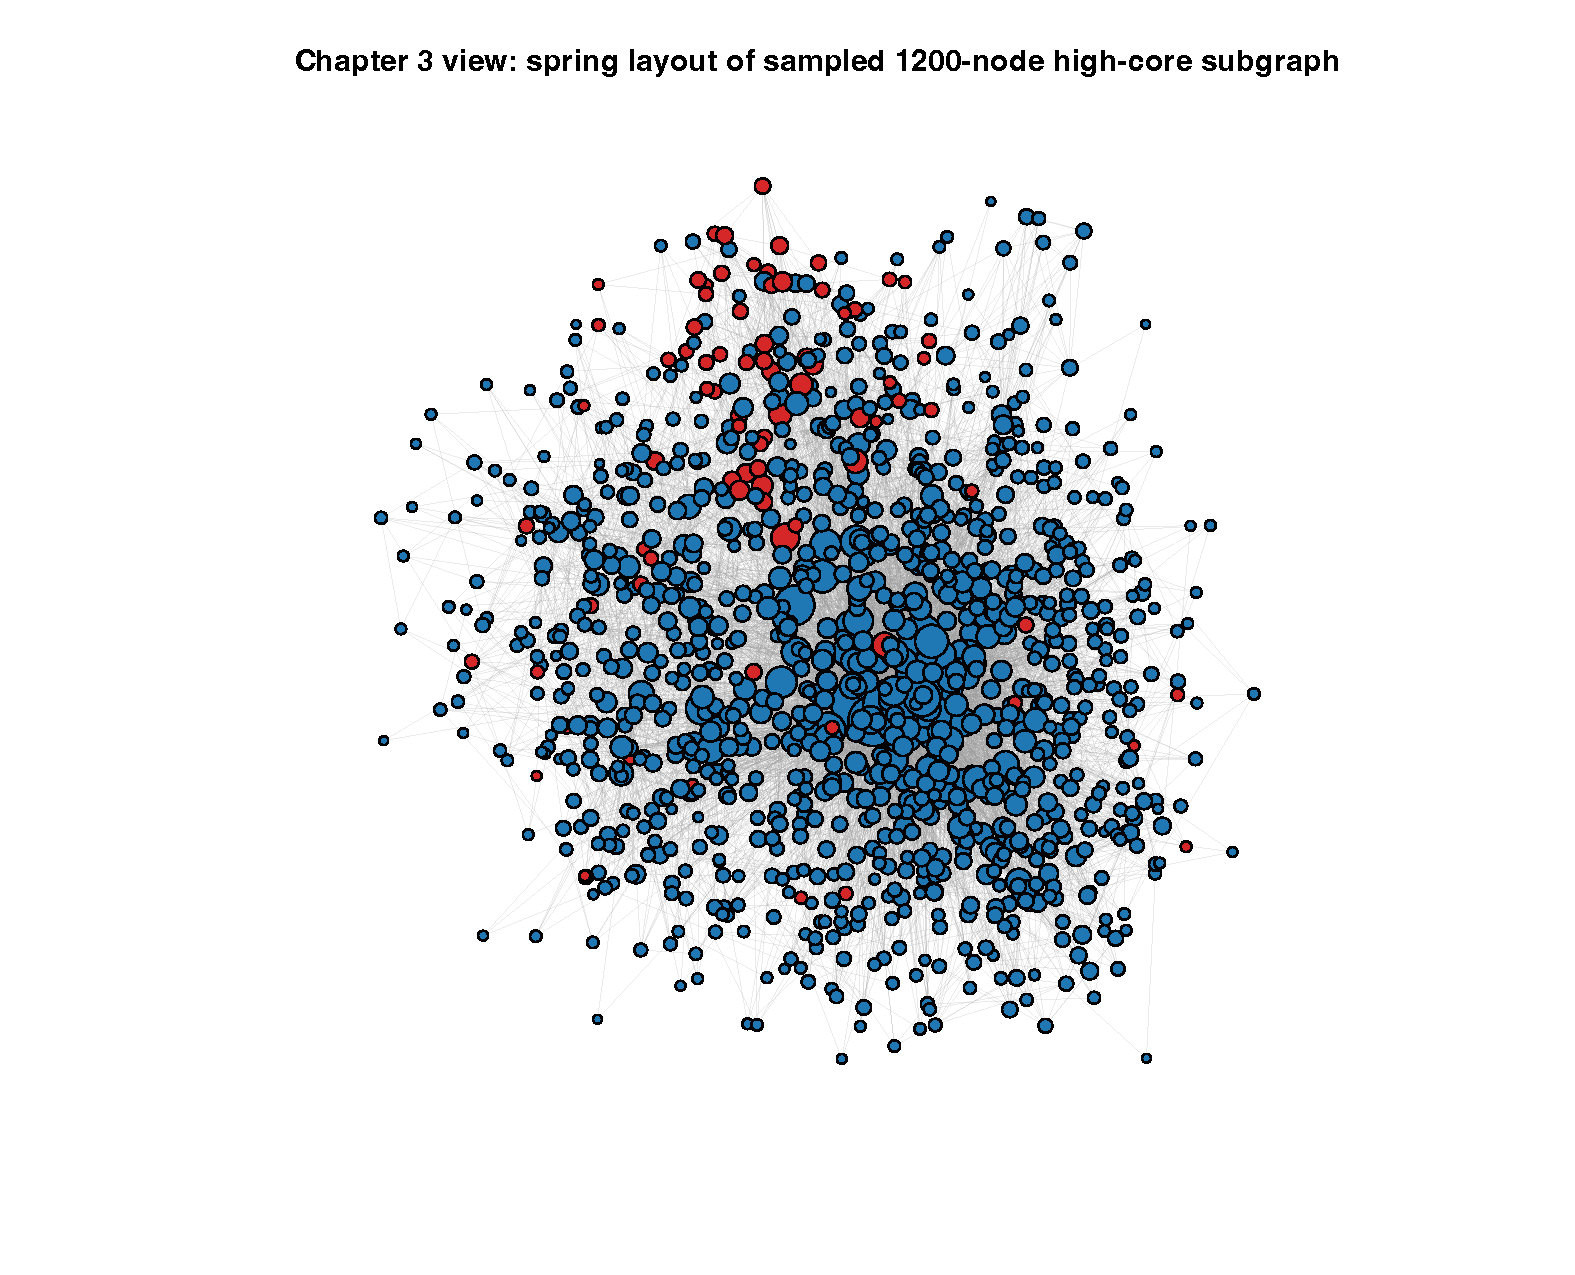
\includegraphics[width=0.85\textwidth]{../codex_outputs/chapter3_layout_high_core.pdf}
  \caption{Spring-embedded layout of the high $k$-core subgraph, revealing the densely connected inner structure of the GitHub network. Nodes in the innermost core ($k=34$) are visible as a tightly clustered region, while nodes in lower $k$-core shells fan outward.}
  \label{fig:high_core}
\end{figure}

What emerges is a clear core--periphery structure: a dense nucleus of elite developers surrounded by progressively sparser layers. Every one of the top 20 hubs from Table~\ref{tab:top_hubs} sits in the innermost core ($k = 33$--$34$), confirming that the most popular developers are not scattered randomly but tightly interconnected with each other.

\subsection{Community-Colored Layout}

\begin{figure}[H]
  \centering
  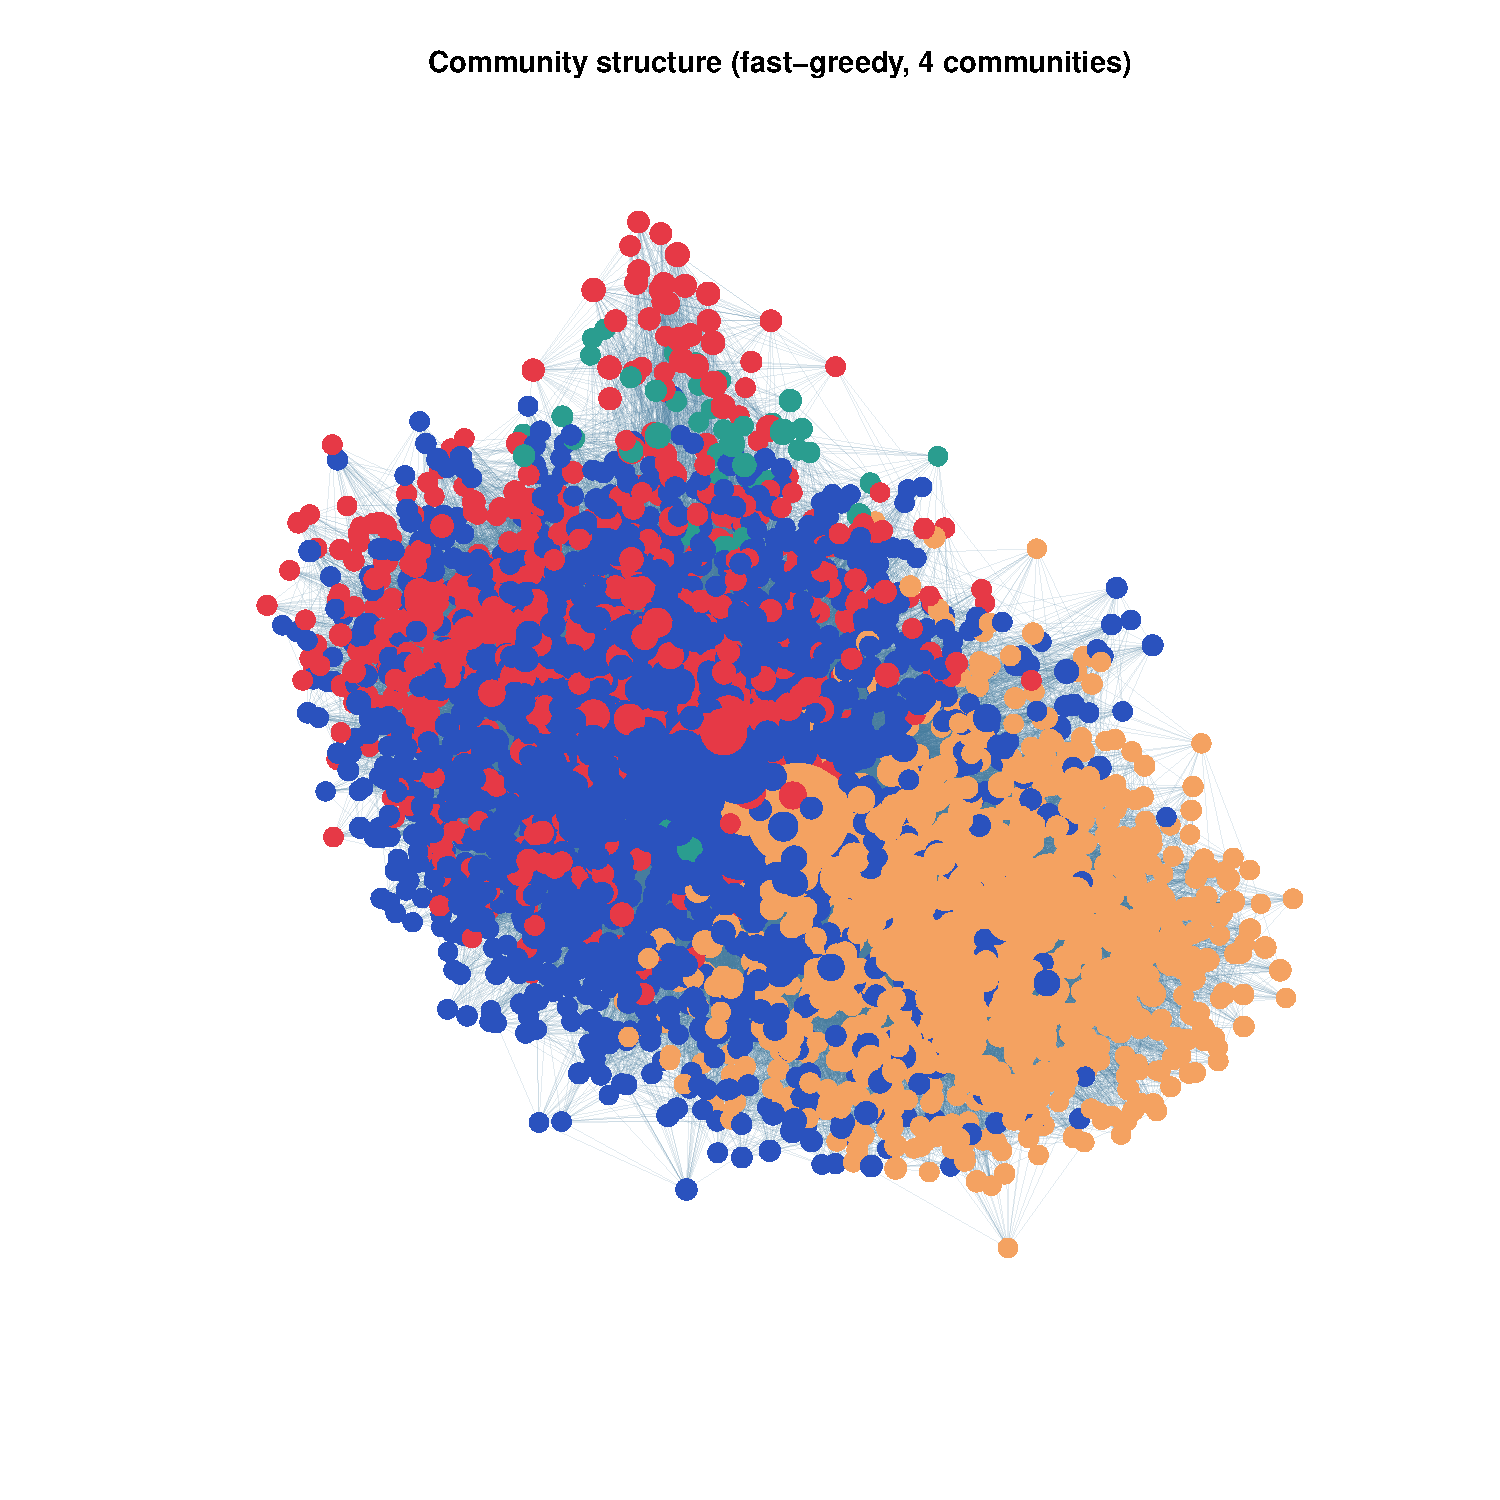
\includegraphics[width=0.85\textwidth]{../claude_analysis/ch3_community_colored.pdf}
  \caption{Network layout with nodes colored by community membership (fast-greedy algorithm). Distinct spatial clusters correspond to different developer communities. The largest communities (containing thousands of nodes each) dominate the visual center, while smaller peripheral communities appear as isolated clusters at the edges.}
  \label{fig:community_colored}
\end{figure}

The community-colored layout reveals that the network partitions into several visually distinct clusters, with the three largest communities (sizes 10,427, 7,908, and 7,597) forming the central mass and numerous smaller communities (median size of just 3 nodes) scattered at the periphery.

\subsection{Ego Network of a Hub Node}

\begin{figure}[H]
  \centering
  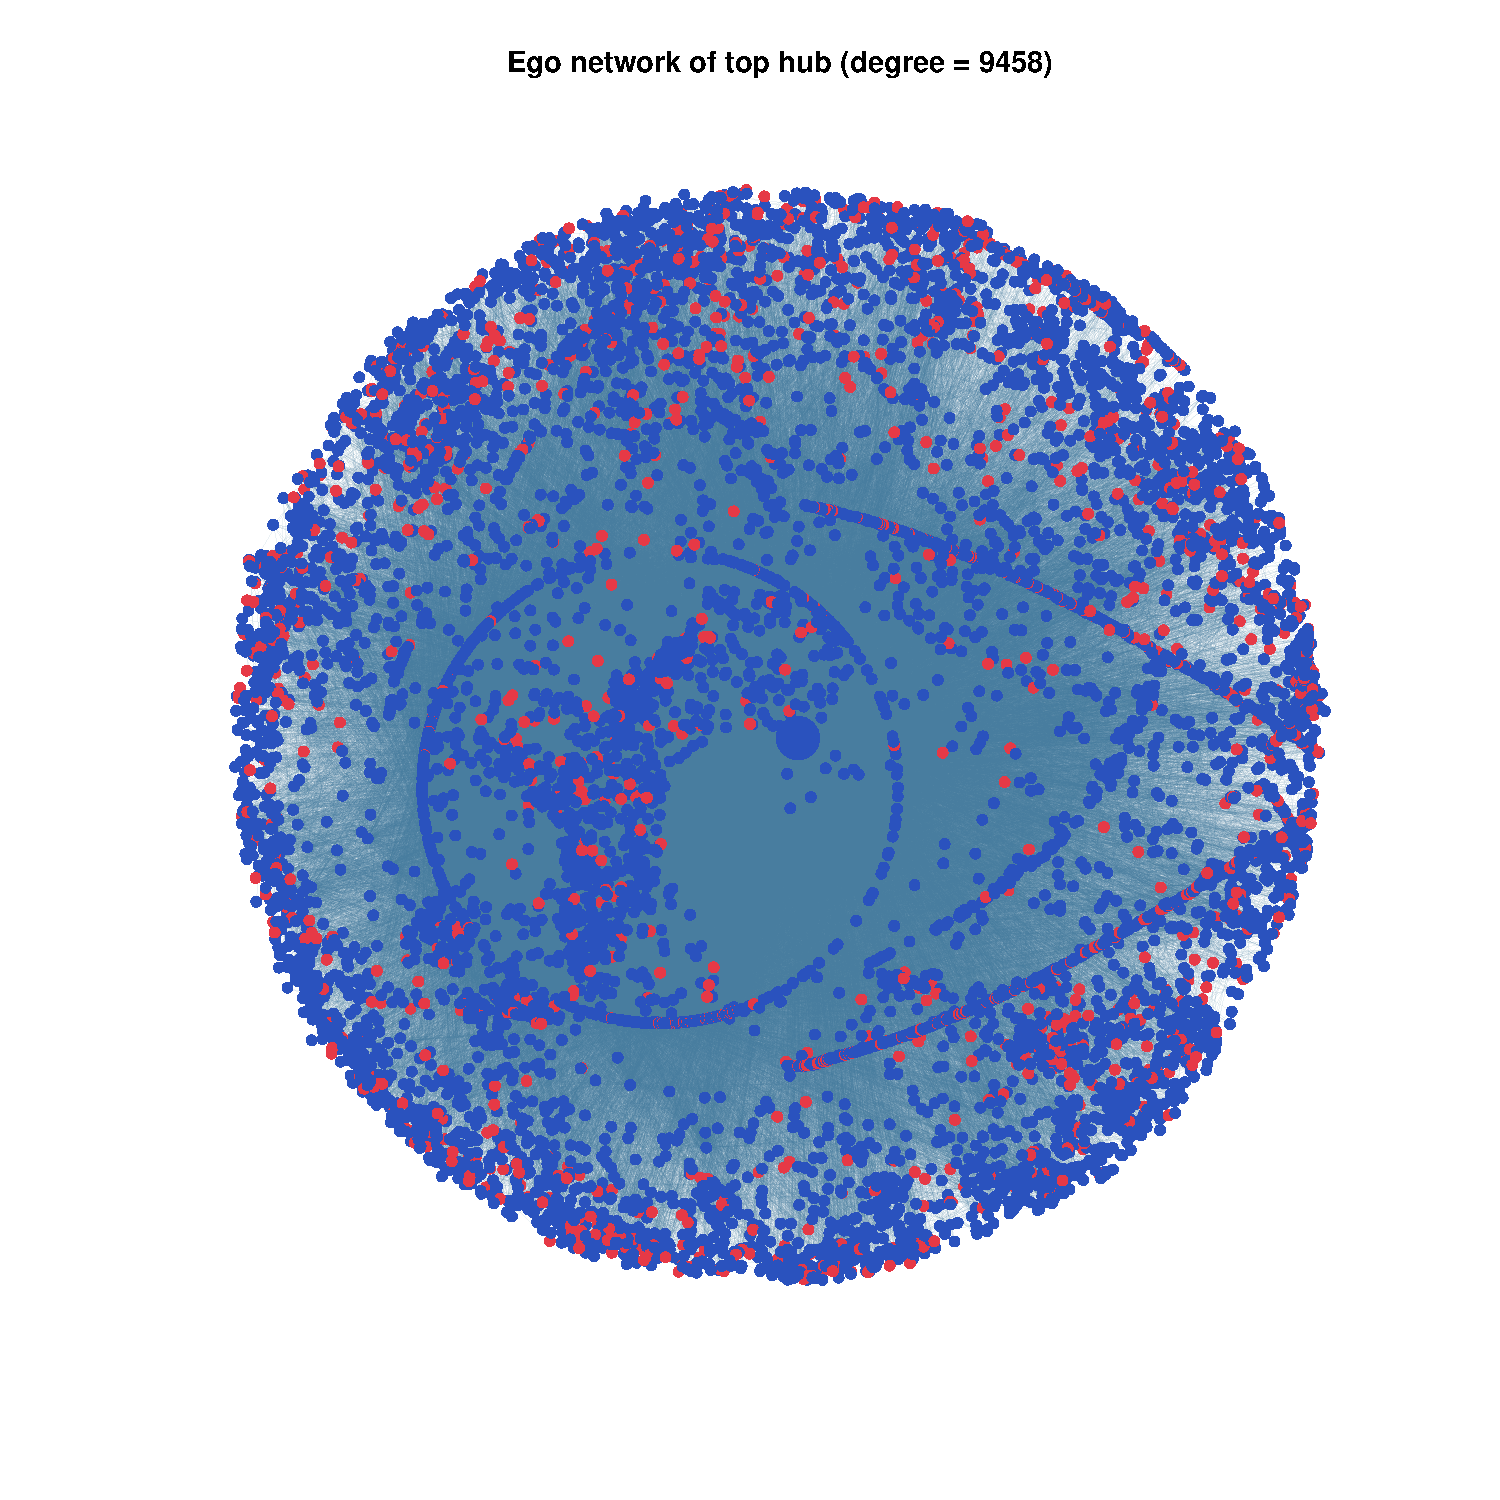
\includegraphics[width=0.7\textwidth]{../claude_analysis/ch3_ego_hub.pdf}
  \caption{Ego network of a major hub node, showing the local neighborhood structure. The hub (center) connects to a large number of alters, many of whom also share connections with each other, forming triangles. The ego network reveals the hub's dual role as both a connector (bridging otherwise unconnected groups) and an aggregator (attracting followers from multiple communities).}
  \label{fig:ego_hub}
\end{figure}

%% ============================================================
\section{Descriptive Analysis}
%% ============================================================

Now we turn to a thorough characterization of the network's structure: who has how many connections, who sits at the center, how tightly clustered are neighborhoods, and what communities exist.

\subsection{Degree Distribution}

The degree distribution---how many connections each developer has---is the single most revealing feature of any network. For the GitHub graph, it tells a story of extreme inequality: most developers have just a handful of followers, while a tiny elite has thousands.

\begin{table}[H]
  \centering
  \begin{tabular}{lrrrrrr}
    \toprule
    \textbf{Mean} & \textbf{Std Dev} & \textbf{Median} & \textbf{Min} & \textbf{Max} & \textbf{P90} & \textbf{P99} \\
    \midrule
    15.33 & 80.79 & 6 & 1 & 9,458 & 30 & 138 \\
    \bottomrule
  \end{tabular}
  \caption{Summary statistics of the node degree distribution.}
  \label{tab:degree_stats}
\end{table}

A few numbers tell the story:
\begin{itemize}
  \item The \textbf{mean} (15.33) is more than $2.5\times$ the \textbf{median} (6), a classic indicator of right-skew caused by high-degree outliers.
  \item The \textbf{standard deviation} (80.79) is $5.3\times$ the mean, indicating enormous variability. Most of this variance comes from a tiny fraction of very high-degree nodes.
  \item The \textbf{90th percentile} is only 30, meaning that 90\% of developers have 30 or fewer mutual followers. Yet the top 1\% have at least 138, and the maximum is 9,458---a range spanning nearly four orders of magnitude.
  \item The \textbf{minimum degree} is 1 (every node has at least one connection, since the graph is connected), confirming that there are no isolated nodes in this particular snapshot.
\end{itemize}

\begin{figure}[H]
  \centering
  \begin{subfigure}[t]{0.48\textwidth}
    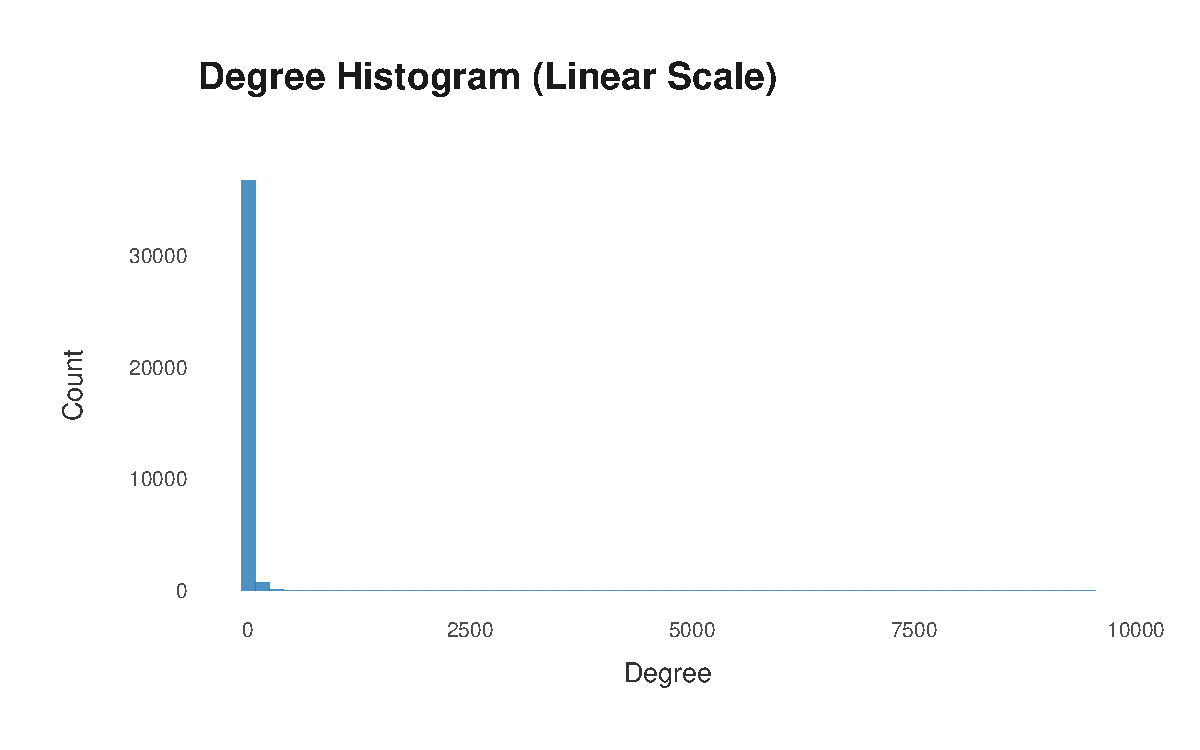
\includegraphics[width=\textwidth]{../codex_outputs/chapter4_degree_hist_linear.pdf}
    \caption{Linear-scale histogram}
  \end{subfigure}
  \hfill
  \begin{subfigure}[t]{0.48\textwidth}
    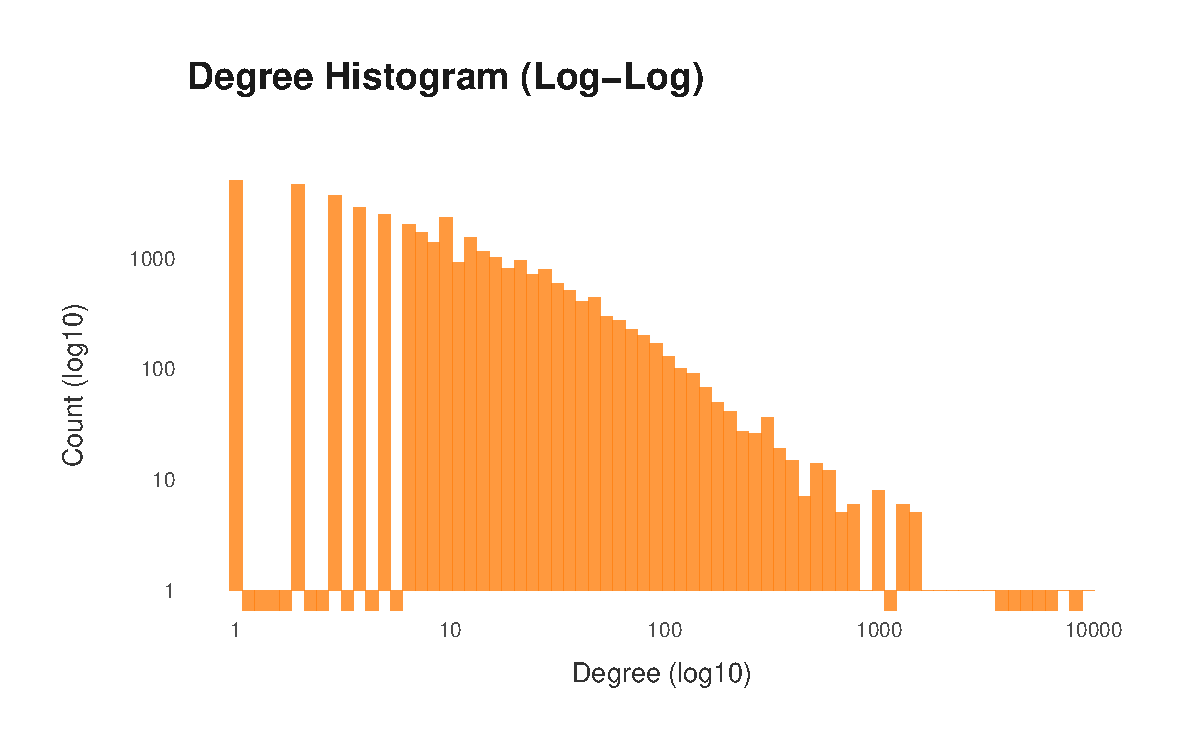
\includegraphics[width=\textwidth]{../codex_outputs/chapter4_degree_hist_log.pdf}
    \caption{Log-scale histogram}
  \end{subfigure}
  \caption{Degree distribution of the GitHub network. The linear plot (a) shows extreme right-skew, with the vast majority of nodes concentrated in the first few bins and a long, barely visible tail. The log-scale plot (b) reveals the structure of the tail more clearly, showing a gradual decay spanning three orders of magnitude.}
  \label{fig:degree_hist}
\end{figure}

\subsubsection{Power-Law Tail Analysis}

Is the tail actually a power law, or just ``heavy''? To find out, we plot the complementary cumulative distribution function (CCDF) on log--log axes. A straight line on this plot is the hallmark of a power law: $P(k) \propto k^{-\gamma}$. Fitting via maximum likelihood gives:
\begin{itemize}
  \item \textbf{Tail exponent}: $\gamma \approx 2.54$
  \item \textbf{Lower cutoff}: $x_{\min} = 55$
\end{itemize}

An exponent of $\gamma \approx 2.54$ places GitHub right in the sweet spot for social networks (most fall between 2 and 3). At this exponent, hubs are common enough to dominate the network's topology, but not so extreme that a single node swallows everything. For context: the World Wide Web sits around $\gamma \approx 2.1$ (even more hub-dominated) and scientific citation networks around $\gamma \approx 3.0$ (more egalitarian). GitHub falls neatly between the two.

\begin{figure}[H]
  \centering
  \begin{subfigure}[t]{0.48\textwidth}
    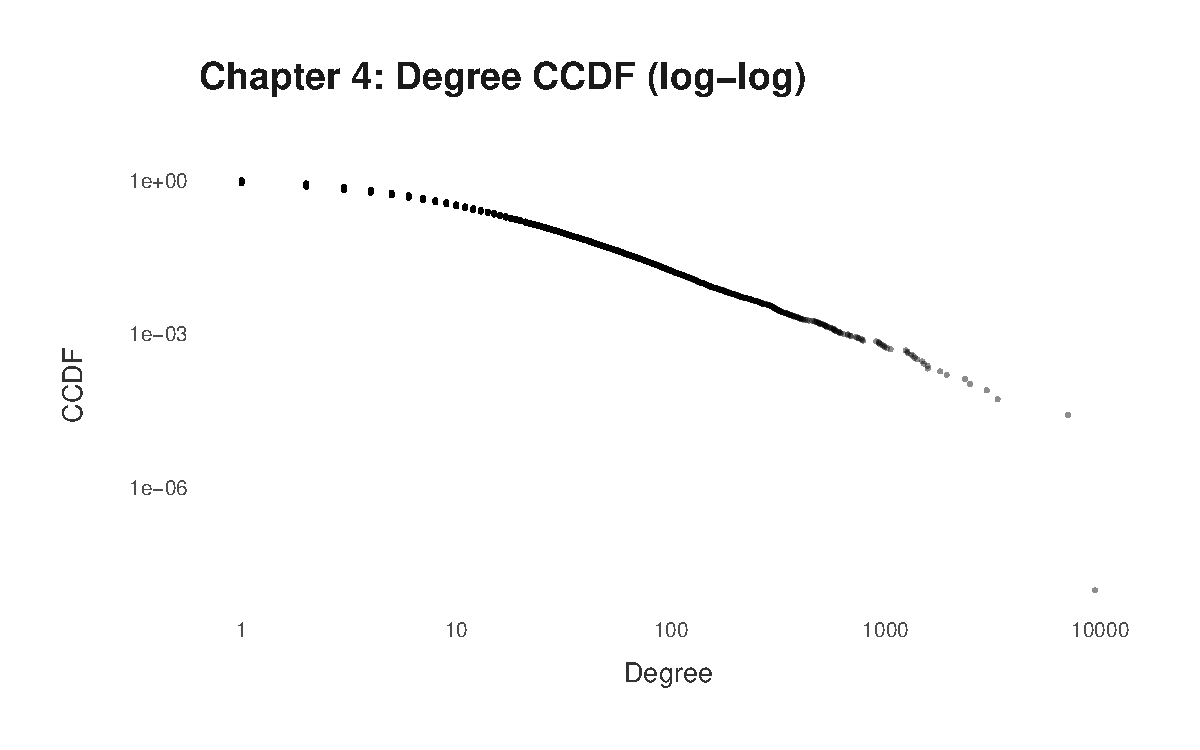
\includegraphics[width=\textwidth]{../codex_outputs/chapter4_degree_ccdf.pdf}
    \caption{CCDF of the degree distribution}
  \end{subfigure}
  \hfill
  \begin{subfigure}[t]{0.48\textwidth}
    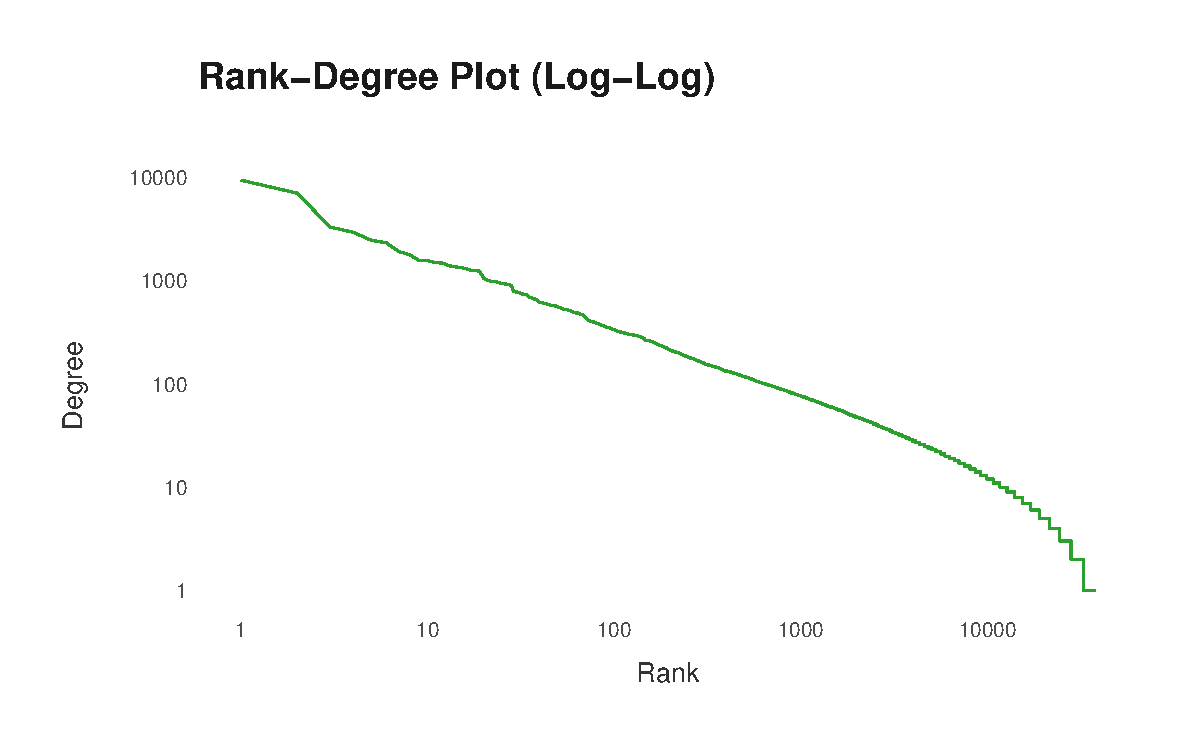
\includegraphics[width=\textwidth]{../codex_outputs/chapter4_rank_degree.pdf}
    \caption{Rank--degree plot}
  \end{subfigure}
  \caption{Power-law behavior in the degree distribution. The CCDF (a) shows an approximately linear region on log--log axes for $k \geq 55$, consistent with a power law with $\gamma \approx 2.54$. The rank--degree plot (b) provides a complementary view: ordering nodes from highest to lowest degree produces the characteristic Zipf-like curve with a steep initial drop followed by a long tail.}
  \label{fig:degree_powerlaw}
\end{figure}

\subsection{Vertex Centrality}

``Importance'' in a network can mean many things: having many connections, sitting at a crossroads, or being close to everyone. We computed five centrality measures---each capturing a different notion of importance---for all 37,700 nodes.

\subsubsection{Full Centrality Table for Top 20 Nodes}

\begin{table}[H]
  \centering
  \small
  \begin{tabular}{rlrrrrr}
    \toprule
    \textbf{Rank} & \textbf{Developer} & \textbf{Degree} & \textbf{Deg.\ Cent.} & \textbf{Closeness} & \textbf{Betweenness} & \textbf{Eigenvec.} \\
    \midrule
    1  & dalinhuang99      & 9,458 & 0.2509 & 0.518 & 0.2696 & 1.0000 \\
    2  & nfultz            & 7,085 & 0.1879 & 0.523 & 0.2405 & 0.8475 \\
    3  & addyosmani        & 3,324 & 0.0882 & 0.450 & 0.0434 & 0.4542 \\
    4  & Bunlong           & 2,958 & 0.0785 & 0.466 & 0.0553 & 0.4182 \\
    5  & gabrielpconceicao & 2,468 & 0.0655 & 0.447 & 0.0353 & 0.3357 \\
    6  & rfthusn           & 2,343 & 0.0622 & 0.440 & 0.0308 & 0.2689 \\
    7  & nelsonic          & 1,924 & 0.0510 & 0.405 & 0.0258 & 0.1552 \\
    8  & getify            & 1,797 & 0.0477 & 0.410 & 0.0175 & 0.2326 \\
    9  & mdo               & 1,571 & 0.0417 & 0.425 & 0.0153 & 0.2285 \\
    10 & ronenhamias       & 1,568 & 0.0416 & 0.442 & 0.0276 & 0.1975 \\
    11 & SuriyaaKudoIsc    & 1,507 & 0.0400 & 0.443 & 0.0189 & 0.2464 \\
    12 & jeresig           & 1,485 & 0.0394 & 0.423 & 0.0102 & 0.2494 \\
    13 & JonnyBanana       & 1,404 & 0.0372 & 0.447 & 0.0203 & 0.2195 \\
    14 & mbostock          & 1,368 & 0.0363 & 0.420 & 0.0133 & 0.2049 \\
    15 & shayan-taheri     & 1,347 & 0.0357 & 0.413 & 0.0213 & 0.1194 \\
    16 & pengliheng        & 1,316 & 0.0349 & 0.421 & 0.0183 & 0.1440 \\
    17 & kentcdodds        & 1,267 & 0.0336 & 0.399 & 0.0095 & 0.1755 \\
    18 & isaacs            & 1,264 & 0.0335 & 0.407 & 0.0071 & 0.2286 \\
    19 & sdras             & 1,240 & 0.0329 & 0.418 & 0.0129 & 0.1633 \\
    20 & kauegimenes       & 1,055 & 0.0280 & 0.425 & 0.0070 & 0.1889 \\
    \bottomrule
  \end{tabular}
  \caption{Complete centrality profile for the top 20 hub nodes. All are Web Developers (class~0) and all reside in $k$-core 33--34.}
  \label{tab:centrality_full}
\end{table}

\subsubsection{Interpretation of Centrality Measures}

\begin{itemize}
  \item \textbf{Degree centrality}: The maximum degree centrality (0.251 for \texttt{dalinhuang99}) is $\sim$617$\times$ the mean (0.000407). This extreme ratio confirms that the network is dominated by a few super-hubs. The top two nodes alone hold normalized degree centralities of 0.251 and 0.188, meaning they connect to 25\% and 19\% of all other nodes, respectively.

  \item \textbf{Closeness centrality}: Closeness values are relatively compressed, ranging from 0.141 (peripheral nodes) to 0.523 (the most central hubs), with a mean of 0.314. The narrow range reflects the small-world property: even peripheral nodes are not far from the center. Notably, \texttt{nfultz} (rank~2) has slightly \emph{higher} closeness (0.523) than \texttt{dalinhuang99} (0.518) despite having fewer connections, suggesting that \texttt{nfultz} is positioned more centrally within the network's geodesic structure.

  \item \textbf{Betweenness centrality}: Most nodes have near-zero betweenness (mean: $5.96 \times 10^{-5}$), but the top two nodes have betweenness of 0.270 and 0.241, meaning they lie on 27\% and 24\% of all shortest paths. These nodes are critical bridges whose removal would substantially increase average path lengths. The sharp drop from rank~2 (0.241) to rank~3 (0.055) reveals that bridging duty is concentrated in just two super-hubs.

  \item \textbf{Eigenvector centrality}: The maximum is 1.000 (by convention, the leading eigenvector is normalized to its largest entry). The top node connects not just to many nodes, but to many \emph{important} nodes---a ``rich club'' effect where hubs preferentially connect to other hubs. The second-highest eigenvector centrality (0.848 for \texttt{nfultz}) confirms this concentration.

  \item \textbf{PageRank}: PageRank scores for the top 20 nodes range from 0.0169 (\texttt{dalinhuang99}) to 0.0015 (\texttt{kauegimenes}). The PageRank rankings largely mirror degree rankings but with some reordering, because PageRank penalizes nodes whose neighbors distribute their ``importance'' across many connections.
\end{itemize}

\begin{figure}[H]
  \centering
  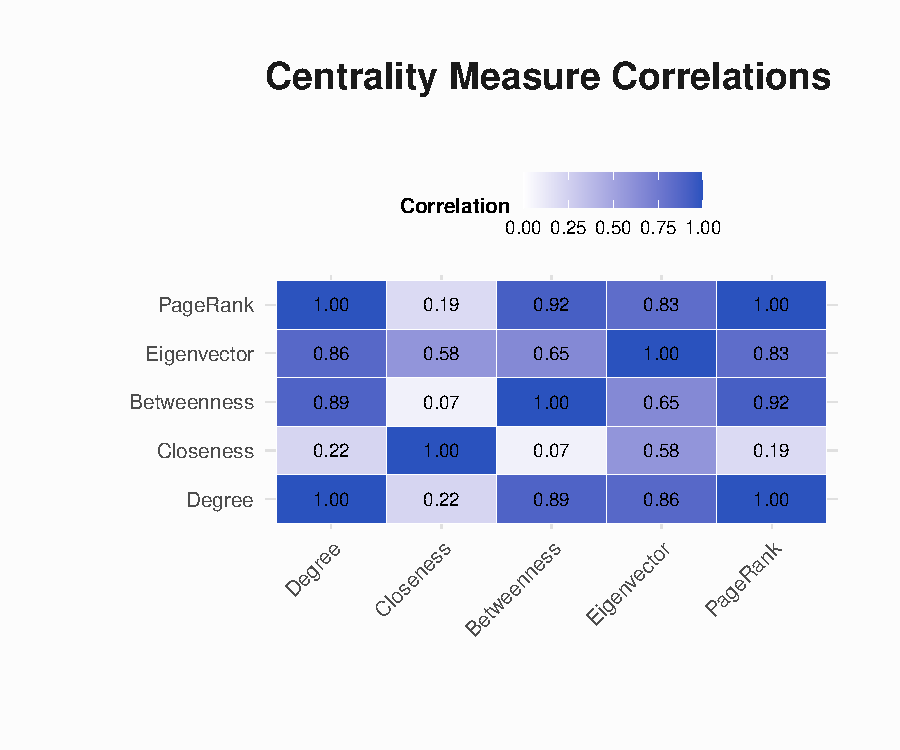
\includegraphics[width=0.75\textwidth]{../claude_analysis/ch4_centrality_correlation.pdf}
  \caption{Pairwise Spearman rank correlation between centrality measures across all 37,700 nodes. Degree and eigenvector centrality are strongly correlated ($\rho > 0.9$), as are degree and betweenness. Closeness centrality shows moderate correlation with the others, reflecting its sensitivity to global network geometry rather than local connectivity alone.}
  \label{fig:centrality_corr}
\end{figure}

\begin{figure}[H]
  \centering
  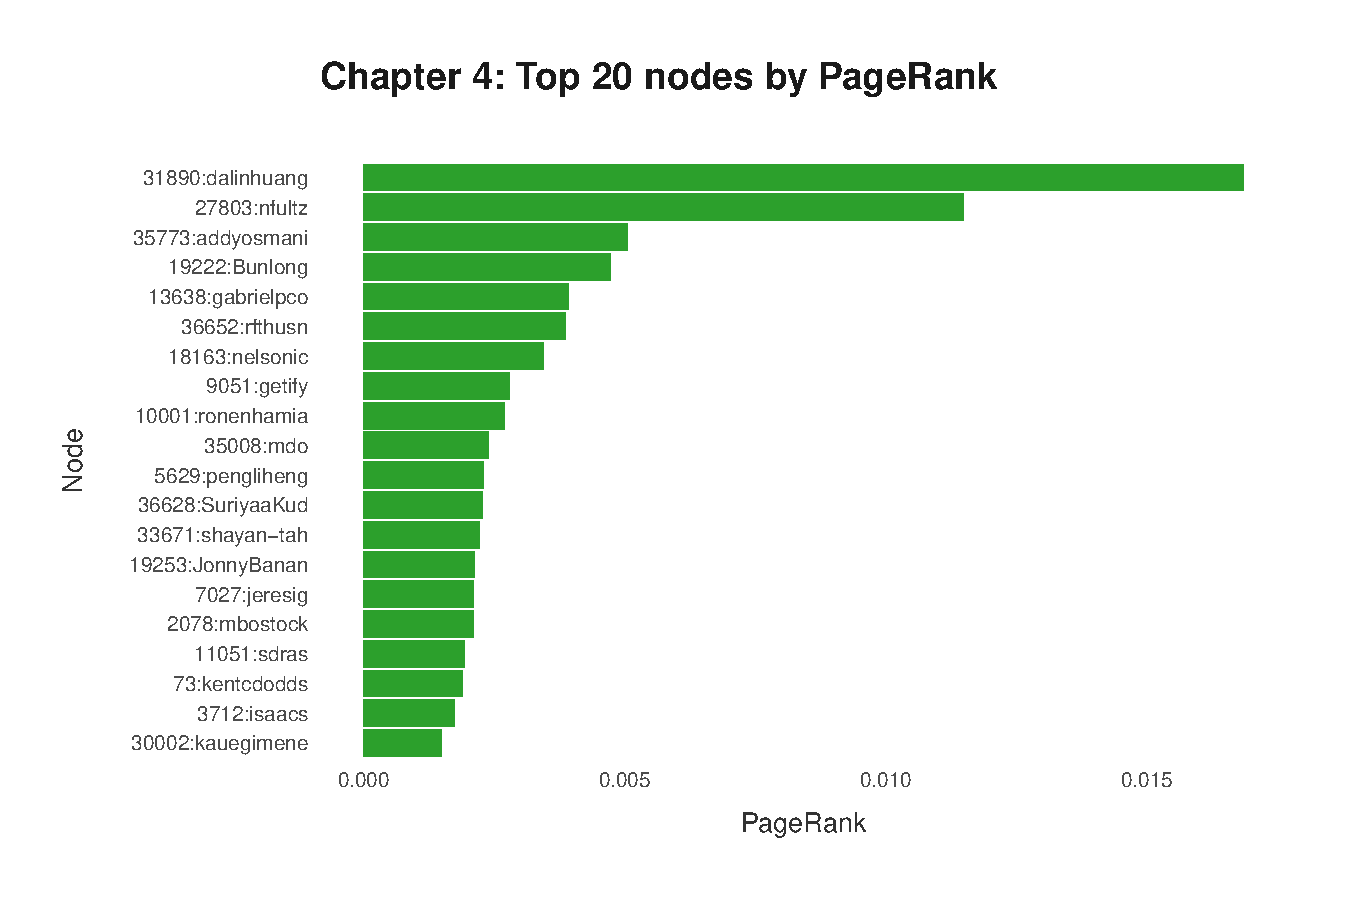
\includegraphics[width=0.75\textwidth]{../codex_outputs/chapter4_top_pagerank.pdf}
  \caption{Top nodes ranked by PageRank. The bar chart shows that PageRank is heavily concentrated in the top few hubs, with a steep drop-off after the first two nodes. This mirrors the degree distribution's heavy tail.}
  \label{fig:pagerank}
\end{figure}

\subsection{Transitivity and Clustering}

If Alice follows Bob and Bob follows Carol, how likely is it that Alice also follows Carol? That is what transitivity (the clustering coefficient) measures---the tendency for triangles to form in the network.

\begin{table}[H]
  \centering
  \begin{tabular}{lrl}
    \toprule
    \textbf{Metric} & \textbf{Value} & \textbf{Interpretation} \\
    \midrule
    Global transitivity    & 0.0124 & Low: sparse triangles globally \\
    Mean local clustering  & 0.1934 & Moderate: tight local neighborhoods \\
    ER expected clustering & 0.000409 & Random baseline for this density \\
    Ratio (global / ER)    & 30.2$\times$ & Far exceeds random expectation \\
    \bottomrule
  \end{tabular}
  \caption{Transitivity measures for the GitHub network, with random graph baseline.}
  \label{tab:transitivity}
\end{table}

The 16-fold gap between global and local clustering reveals something interesting: the network as a whole has sparse triangles, but individual neighborhoods can be quite tightly knit. Think of it this way---if you are a low-degree developer who follows 5 people, those 5 probably know each other (high local clustering). But if you are a hub with 3,000 followers, those followers are drawn from all corners of the network and mostly have nothing to do with each other (low local clustering). This is the characteristic clustering profile of a scale-free network.

\begin{figure}[H]
  \centering
  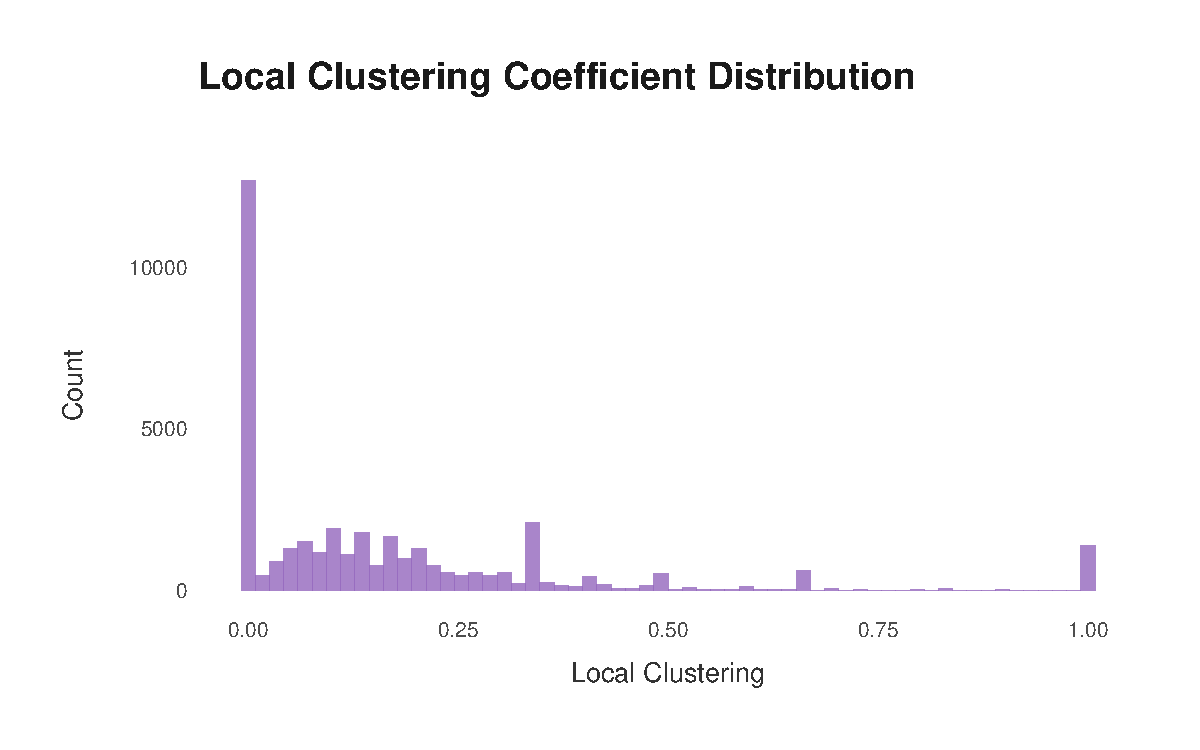
\includegraphics[width=0.75\textwidth]{../codex_outputs/chapter4_local_clustering.pdf}
  \caption{Distribution of local clustering coefficients across all nodes. The bimodal-like structure shows a large mass near zero (hub nodes and low-degree nodes with no triangles) and a secondary concentration at moderate-to-high values (peripheral nodes embedded in tight-knit groups).}
  \label{fig:local_clustering}
\end{figure}

\subsection{$k$-Core Decomposition}

Imagine peeling an onion: remove the outermost, most loosely connected nodes first, then the next layer, and so on. The $k$-core decomposition does exactly this---the $k$-core is the largest subgraph where every remaining node has at least $k$ connections to other remaining nodes. For the GitHub network:

\begin{itemize}
  \item The \textbf{maximum coreness} is $k = 34$, meaning there exists a subgraph where every node has at least 34 connections to other members of that subgraph.
  \item All 20 top hub nodes (Table~\ref{tab:centrality_full}) reside in $k$-core 33--34, confirming that the most connected developers form a tightly interconnected elite.
  \item The majority of nodes reside in low-$k$ shells ($k = 1$--5), reflecting the predominance of loosely connected peripheral developers.
\end{itemize}

\begin{figure}[H]
  \centering
  \begin{subfigure}[t]{0.48\textwidth}
    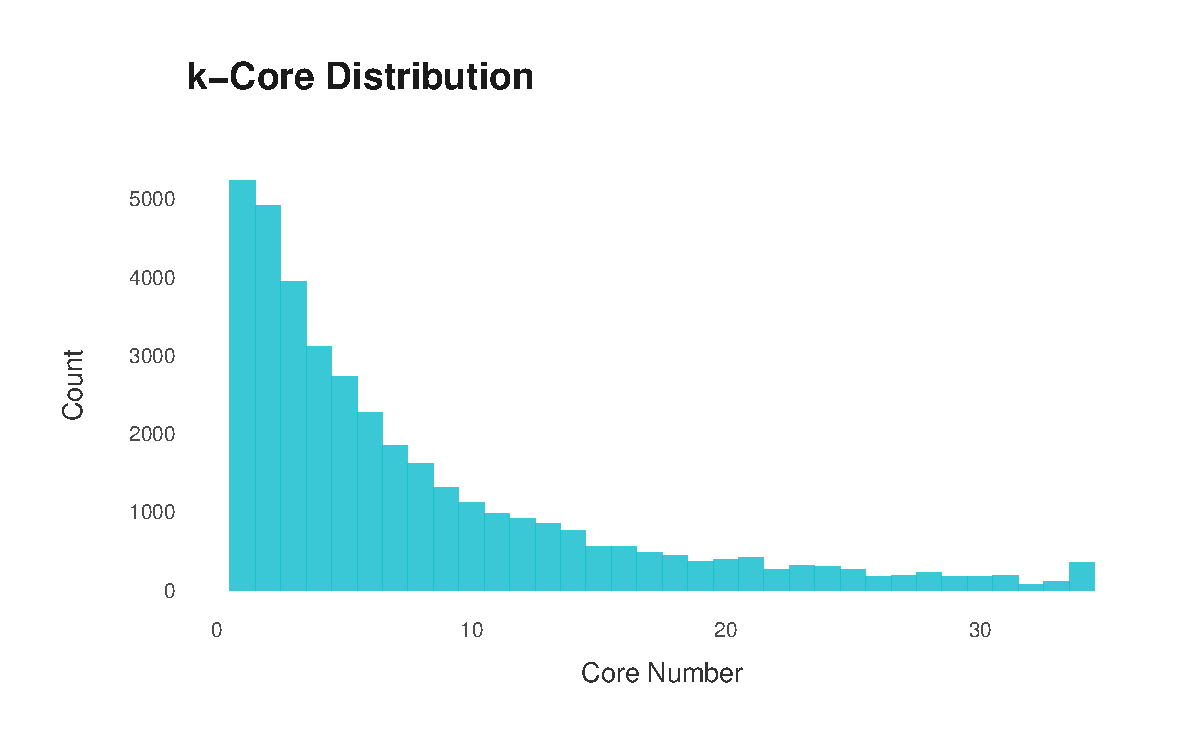
\includegraphics[width=\textwidth]{../codex_outputs/chapter4_core_distribution.pdf}
    \caption{Distribution of $k$-core numbers}
  \end{subfigure}
  \hfill
  \begin{subfigure}[t]{0.48\textwidth}
    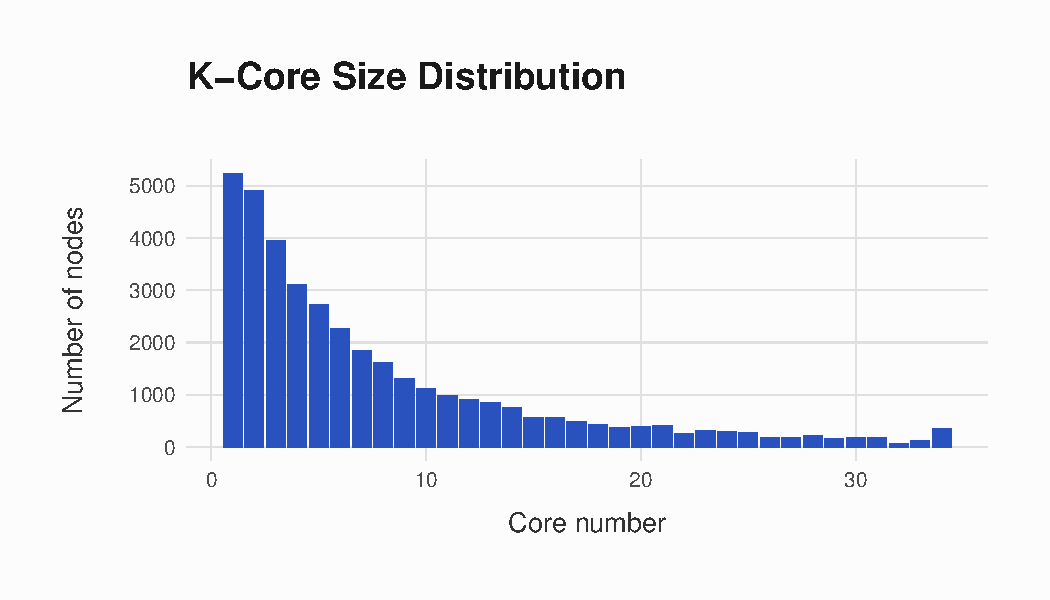
\includegraphics[width=\textwidth]{../claude_analysis/ch4_kcore_distribution.pdf}
    \caption{$k$-core size by shell}
  \end{subfigure}
  \caption{$k$-core decomposition of the GitHub network. Panel (a) shows that most nodes are in low-$k$ shells, with a long tail extending to $k = 34$. Panel (b) shows the number of nodes at each coreness level, revealing the core--periphery structure.}
  \label{fig:kcore}
\end{figure}

\subsection{Community Detection}

Are there natural ``neighborhoods'' in this network---groups of developers who follow each other much more than they follow outsiders? To find out, we ran the fast-greedy community detection algorithm, which greedily merges groups to maximize Newman's modularity $Q$ (a score from 0 to 1 measuring how much denser within-community edges are compared to random).

\begin{table}[H]
  \centering
  \begin{tabular}{lr}
    \toprule
    \textbf{Metric} & \textbf{Value} \\
    \midrule
    Number of communities & 85 \\
    Modularity $Q$        & 0.453 \\
    Largest community     & 10,427 nodes (27.7\%) \\
    2nd largest           & 7,908 nodes (21.0\%) \\
    3rd largest           & 7,597 nodes (20.2\%) \\
    4th largest           & 3,338 nodes (8.9\%) \\
    5th largest           & 3,173 nodes (8.4\%) \\
    Median community size & 3 nodes \\
    Smallest communities  & 2 nodes (many) \\
    \bottomrule
  \end{tabular}
  \caption{Community detection summary (fast-greedy algorithm). The top 5 communities contain 86\% of all nodes.}
  \label{tab:community_summary}
\end{table}

A modularity of $Q = 0.453$ is well above the 0.3 threshold that network scientists typically consider ``meaningful.'' But the community sizes are wildly unequal: the top three communities alone swallow 69\% of all developers, while the remaining 82 communities account for just 31\%. Even the community structure follows a power law---the network is hierarchical all the way down.

\begin{table}[H]
  \centering
  \begin{tabular}{rr|rr|rr}
    \toprule
    \textbf{Community} & \textbf{Size} & \textbf{Community} & \textbf{Size} & \textbf{Community} & \textbf{Size} \\
    \midrule
    4  & 10,427 & 1  & 1,960 & 10 & 458 \\
    3  & 7,908  & 9  & 1,198 & 13 & 261 \\
    2  & 7,597  & 5  & 562   & 11 & 239 \\
    6  & 3,338  & --- & ---  & 12 & 180 \\
    8  & 3,173  & --- & ---  & 7  & 93  \\
    \bottomrule
  \end{tabular}
  \caption{Sizes of the top 15 communities. The remaining 70 communities have sizes ranging from 2 to 54 nodes.}
  \label{tab:community_sizes_detail}
\end{table}

\begin{figure}[H]
  \centering
  \includegraphics[width=0.75\textwidth]{../codex_outputs/chapter4_community_sizes.pdf}
  \caption{Community size distribution (log scale). A few large communities dominate, while the long tail of small communities reflects micro-clusters of 2--5 developers who follow each other but have limited external connections.}
  \label{fig:community_sizes}
\end{figure}

\subsection{Assortativity and Mixing Patterns}

Do birds of a feather flock together on GitHub? Assortativity measures exactly this: the tendency for similar nodes to connect. We look at two dimensions---degree (do popular developers follow other popular developers?) and profession (do ML engineers follow other ML engineers?).

\begin{table}[H]
  \centering
  \begin{tabular}{lrl}
    \toprule
    \textbf{Assortativity} & \textbf{Value} & \textbf{Interpretation} \\
    \midrule
    Degree                 & $-0.075$ & Mildly disassortative (hubs $\to$ periphery) \\
    ML\_target (homophily)  & $+0.378$ & Strongly assortative (same type $\to$ same type) \\
    \bottomrule
  \end{tabular}
  \caption{Assortativity coefficients.}
  \label{tab:assortativity}
\end{table}

The answer is nuanced. For degree, the answer is \emph{no}: the negative coefficient ($r = -0.075$) tells us that popular developers mostly attract followers from the vast pool of ordinary users, not from each other. It is a hub-and-spoke pattern---the popular kids are friends with everyone, not just with each other.

But for profession, the answer is a resounding \emph{yes}: the strong positive coefficient ($r = 0.378$) means ML engineers disproportionately follow other ML engineers, and Web Developers follow other Web Developers. This is genuine homophily---professional birds of a feather really do flock together on GitHub. The mixing matrix makes this concrete:

\begin{table}[H]
  \centering
  \begin{tabular}{l|rr|r}
    \toprule
    & \textbf{Web (0)} & \textbf{MLE (1)} & \textbf{Total} \\
    \midrule
    \textbf{Web (0)} & 224,623 (77.7\%) & 44,696 (15.5\%) & 269,319 \\
    \textbf{MLE (1)} & 44,696 (15.5\%)  & 19,684 (6.8\%)  & 64,380  \\
    \midrule
    \textbf{Total}   & 269,319          & 64,380           & \textbf{289,003 (2$\times$)} \\
    \bottomrule
  \end{tabular}
  \caption{Edge mixing matrix by developer type (each undirected edge counted once). Percentages show the fraction of total edges.}
  \label{tab:mixing}
\end{table}

\begin{figure}[H]
  \centering
  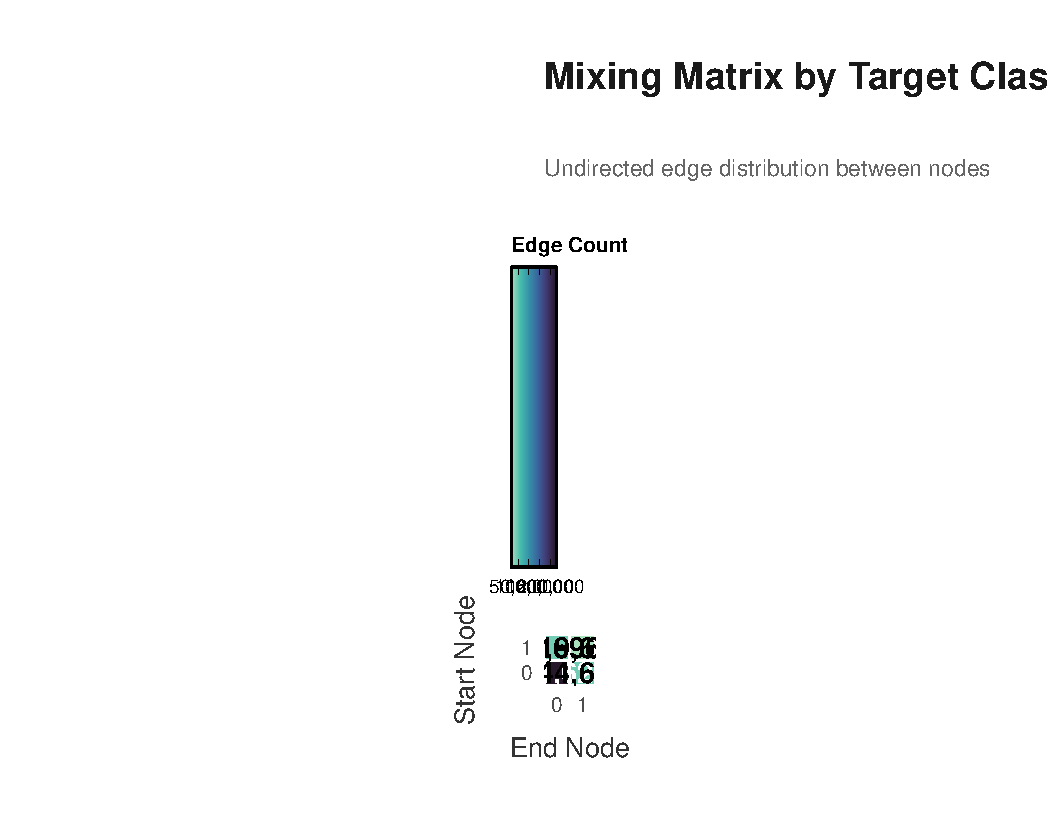
\includegraphics[width=0.6\textwidth]{../codex_outputs/chapter4_mixing_heatmap.pdf}
  \caption{Heatmap of the mixing matrix. The dominant diagonal entries reflect strong within-group connectivity (homophily), while the off-diagonal entries represent cross-type connections.}
  \label{fig:mixing_heatmap}
\end{figure}

But wait---couldn't this just be a base-rate effect? There are 3$\times$ more Web Developers, so of course most edges are Web--Web. To check, we compute the edge \emph{probability} for each block pair (edges observed divided by possible pairs). If type did not matter, all three probabilities would be roughly equal. They are not:

\begin{table}[H]
  \centering
  \begin{tabular}{lrrr}
    \toprule
    \textbf{Block Pair} & \textbf{Possible Pairs} & \textbf{Edge Count} & \textbf{Edge Prob.} \\
    \midrule
    Web--Web   & 390,894,780 & 224,623 & $5.75 \times 10^{-4}$ \\
    Web--MLE   & 272,312,179 & 44,696  & $1.64 \times 10^{-4}$ \\
    MLE--MLE   & 47,419,191  & 19,684  & $4.15 \times 10^{-4}$ \\
    \bottomrule
  \end{tabular}
  \caption{Stochastic block model edge probabilities. Within-group probabilities exceed the cross-group probability by 2.5--3.5$\times$.}
  \label{tab:block_probs}
\end{table}

The Web--Web edge probability ($5.75 \times 10^{-4}$) is $3.5\times$ the cross-type probability ($1.64 \times 10^{-4}$), and the MLE--MLE probability ($4.15 \times 10^{-4}$) is $2.5\times$ the cross-type probability. This confirms that homophily is a real structural feature of the network, not an artifact of group sizes.

\subsubsection{Latent Drivers of Connectivity}

Beyond job titles, other attributes act as powerful latent drivers of homophily. Developers within the same organization have a significantly higher probability of forming mutual follower ties, creating dense pockets of connectivity within the larger graph. Similarly, despite the global nature of open-source, geographic proximity remains a factor: developers in metropolitan technical hubs (San Francisco, London, Bangalore) form tighter clusters than those in more isolated regions.

\subsubsection{Tie Dissolution and Unfollowing}

The network is not static; edges are also removed over time. Longitudinal analysis of GitHub data~\cite{yu2023unfollowing} suggests that ``unfollowing'' is often driven by a lack of activity or a divergence in technical interests. Developers are more likely to unfollow peers who have lower programming language similarity or who decrease their commit frequency. Mutual follower relationships are significantly more resilient to dissolution, with an estimated 60\% lower chance of breaking compared to asymmetric relationships. This stability reinforces the idea that mutual follows represent a form of social capital that developers are hesitant to discard.

\subsection{Spectral Analysis}

The graph Laplacian $L = D - A$ (degree matrix minus adjacency matrix) translates the network's connectivity into a spectrum of eigenvalues---numbers that encode everything from basic connectivity to community structure to how quickly information diffuses across the network.

\begin{table}[H]
  \centering
  \begin{tabular}{lrl}
    \toprule
    \textbf{Spectral Metric} & \textbf{Value} & \textbf{Interpretation} \\
    \midrule
    Smallest eigenvalue ($\lambda_1$) & $\approx 0$ & Confirms connectivity (one component) \\
    Fiedler value ($\lambda_2$)       & 0.117 & Moderate algebraic connectivity \\
    $\lambda_3$                       & 0.156 & Gap $\lambda_3 - \lambda_2 = 0.040$ \\
    $\lambda_4$                       & 0.158 & Cluster of eigenvalues near 0.16--0.20 \\
    Largest eigenvalue ($\lambda_n$)  & 9,459 & Driven by max degree ($\approx 9458 + 1$) \\
    Spectral gap (top)                & 2,373 & Large gap reflects degree heterogeneity \\
    Near-zero eigenvalues             & 1     & Single connected component \\
    \bottomrule
  \end{tabular}
  \caption{Summary of the Laplacian spectrum. The Fiedler value, gap structure, and largest eigenvalue each carry distinct information about network organization.}
  \label{tab:laplacian}
\end{table}

\subsubsection{Interpreting the Spectrum}

The Fiedler value ($\lambda_2 = 0.117$) is the algebraic connectivity of the graph---it quantifies how tightly connected the network is. A value of 0.117 indicates moderate connectivity: the network holds together, but not robustly. In comparison, a complete graph on $n$ nodes has $\lambda_2 = n$, and a cycle graph has $\lambda_2 \approx 2(1 - \cos(2\pi/n)) \approx 0$. The GitHub network falls between these extremes, closer to the sparse end.

The cluster of small eigenvalues near 0.16--0.20 ($\lambda_3$ through $\lambda_{11}$ all lie between 0.156 and 0.199) suggests the presence of approximately 5--10 well-separated communities, consistent with the community detection results showing 5 large communities containing 86\% of nodes.

The largest eigenvalues are approximately equal to $d_i + 1$ for the highest-degree nodes, confirming that the top of the spectrum is driven by the hub structure. The gap of 2,373 between the largest and second-largest eigenvalues reflects the extreme separation between the top hub's degree (9,458) and the second hub's degree (7,085).

\begin{table}[H]
  \centering
  \begin{tabular}{rr|rr}
    \toprule
    \textbf{Index} & \textbf{Eigenvalue} & \textbf{Index} & \textbf{Eigenvalue} \\
    \midrule
    1  & $\approx 0$  & 7  & 0.195 \\
    2  & 0.117        & 8  & 0.197 \\
    3  & 0.156        & 9  & 0.198 \\
    4  & 0.158        & 10 & 0.198 \\
    5  & 0.183        & 11 & 0.198 \\
    6  & 0.190        & 12 & 0.229 \\
    \bottomrule
  \end{tabular}
  \caption{The 12 smallest Laplacian eigenvalues. The single near-zero eigenvalue confirms connectivity; the cluster near 0.16--0.20 relates to community structure.}
  \label{tab:eigenvalues_small}
\end{table}

\begin{figure}[H]
  \centering
  \begin{subfigure}[t]{0.48\textwidth}
    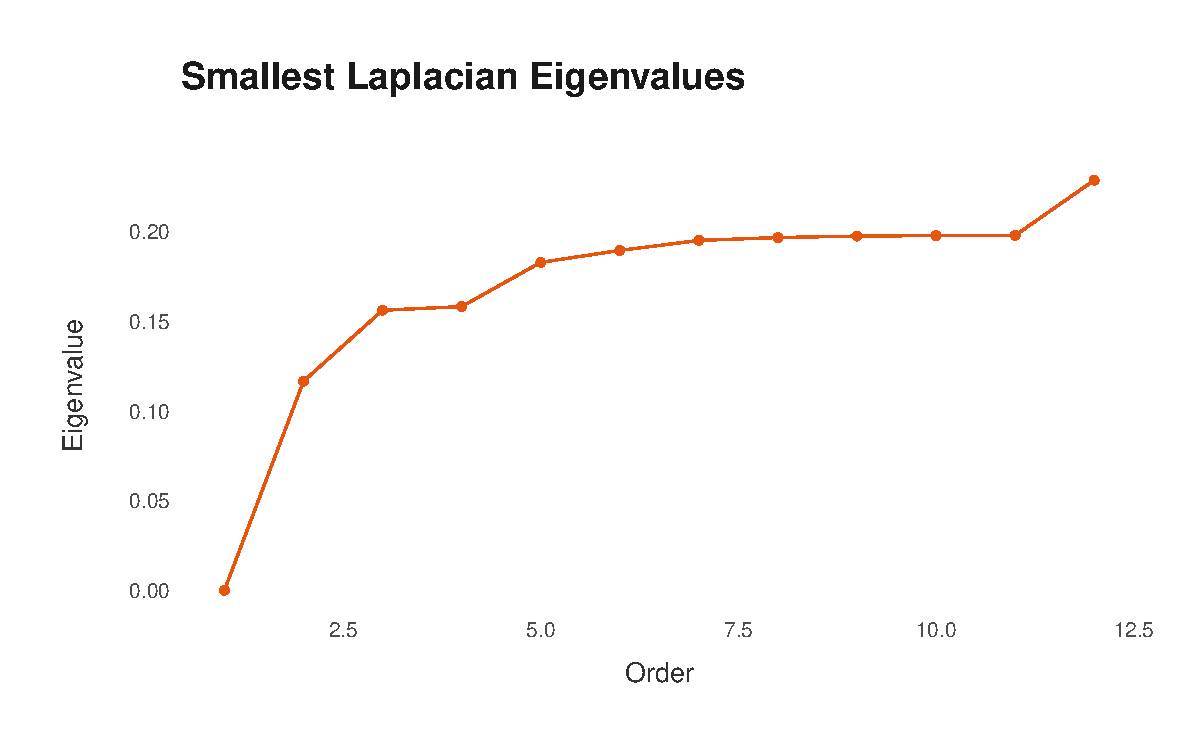
\includegraphics[width=\textwidth]{../codex_outputs/chapter4_laplacian_smallest_plot.pdf}
    \caption{Smallest eigenvalues of the full graph}
  \end{subfigure}
  \hfill
  \begin{subfigure}[t]{0.48\textwidth}
    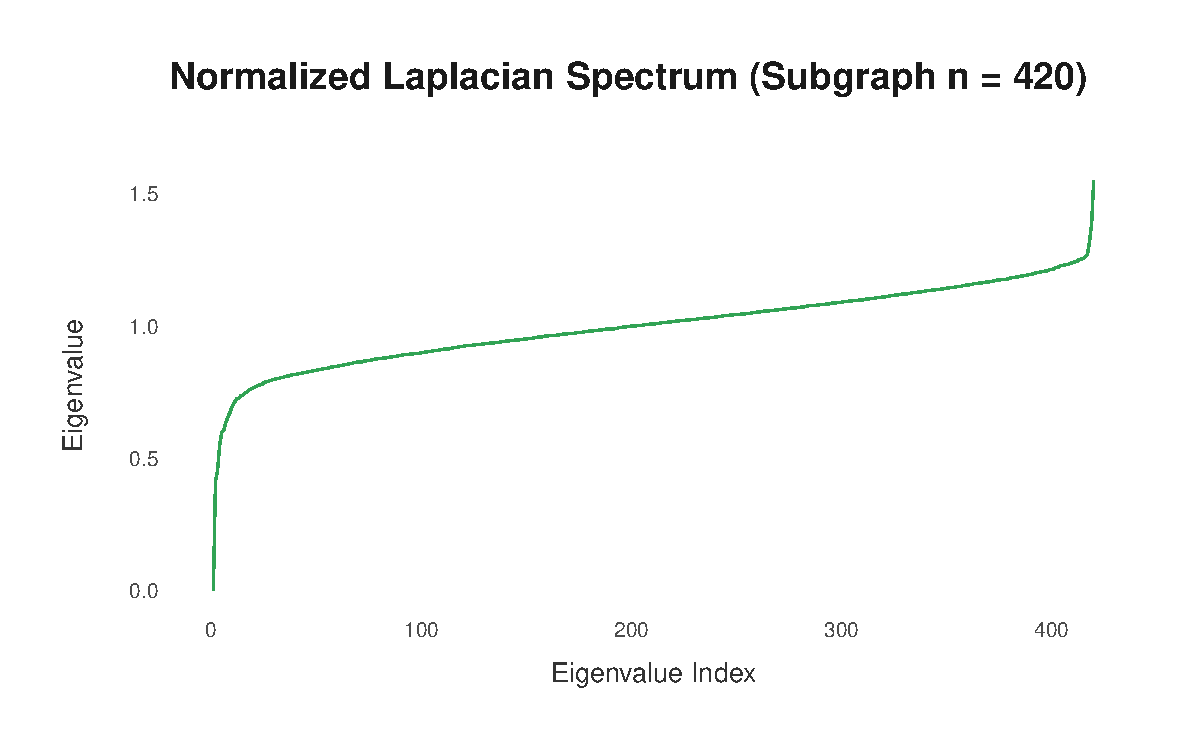
\includegraphics[width=\textwidth]{../codex_outputs/chapter4_laplacian_subgraph_spectrum.pdf}
    \caption{Full spectrum of a tractable subgraph}
  \end{subfigure}
  \caption{Laplacian spectral analysis. Panel (a) shows the smallest eigenvalues from the full 37,700-node graph, computed via sparse eigensolvers (RSpectra). Panel (b) shows the complete spectrum of a smaller subgraph (420 nodes), revealing the full eigenvalue distribution from near-zero to approximately 1.55.}
  \label{fig:laplacian}
\end{figure}

\subsection{Hierarchical Clustering}

Modularity-based methods find flat partitions, but real communities are often nested: small teams inside departments inside organizations. Hierarchical clustering captures this nesting by building a dendrogram---a tree that shows how communities merge at progressively coarser scales. The catch is that it requires an $O(n^2)$ distance matrix, which is infeasible for 37,700 nodes. We therefore applied it to a tractable 180-node subgraph extracted from the high $k$-core.

\begin{table}[H]
  \centering
  \begin{tabular}{rr}
    \toprule
    \textbf{Cluster} & \textbf{Size} \\
    \midrule
    5 & 77 \\
    1 & 56 \\
    2 & 23 \\
    4 & 12 \\
    3 & 8  \\
    6 & 4  \\
    \bottomrule
  \end{tabular}
  \caption{Cluster sizes from hierarchical clustering of the high $k$-core subgraph (6 clusters, 180 nodes total).}
  \label{tab:hclust}
\end{table}

\begin{figure}[H]
  \centering
  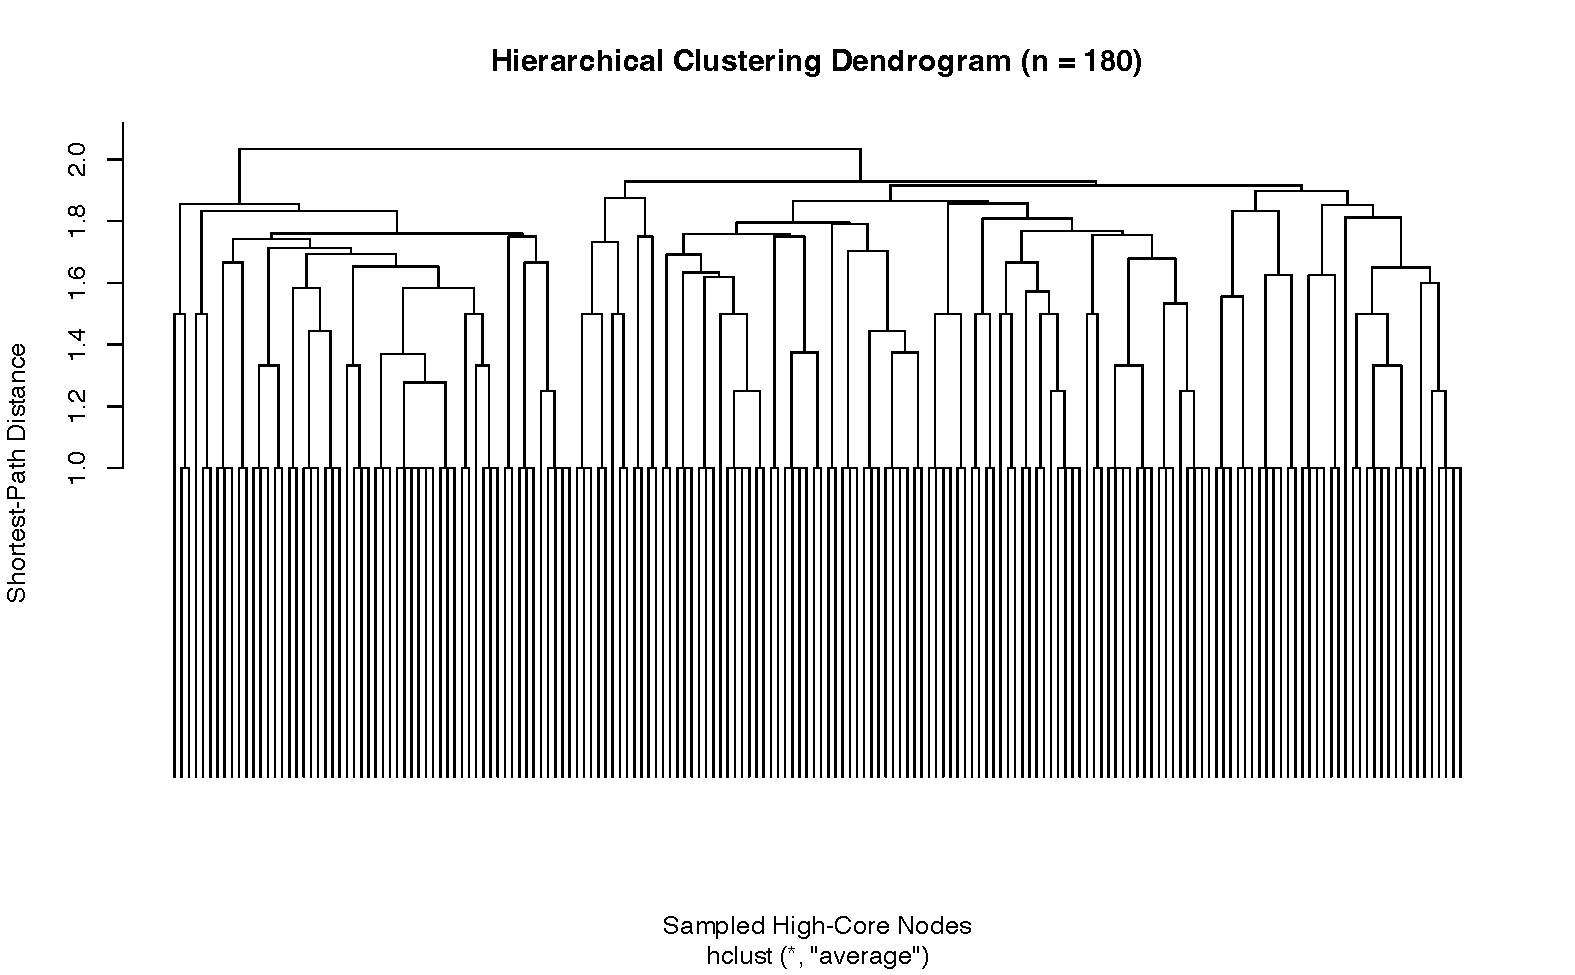
\includegraphics[width=0.85\textwidth]{../codex_outputs/chapter4_hclust_dendrogram.pdf}
  \caption{Dendrogram from hierarchical clustering of the high $k$-core subgraph. The tree reveals nested community structure: a large group of 77 nodes (cluster~5) and another of 56 (cluster~1) are the dominant subcommunities within the core, while smaller satellite clusters (sizes 4--23) branch off at earlier merge heights.}
  \label{fig:dendrogram}
\end{figure}

\begin{figure}[H]
  \centering
  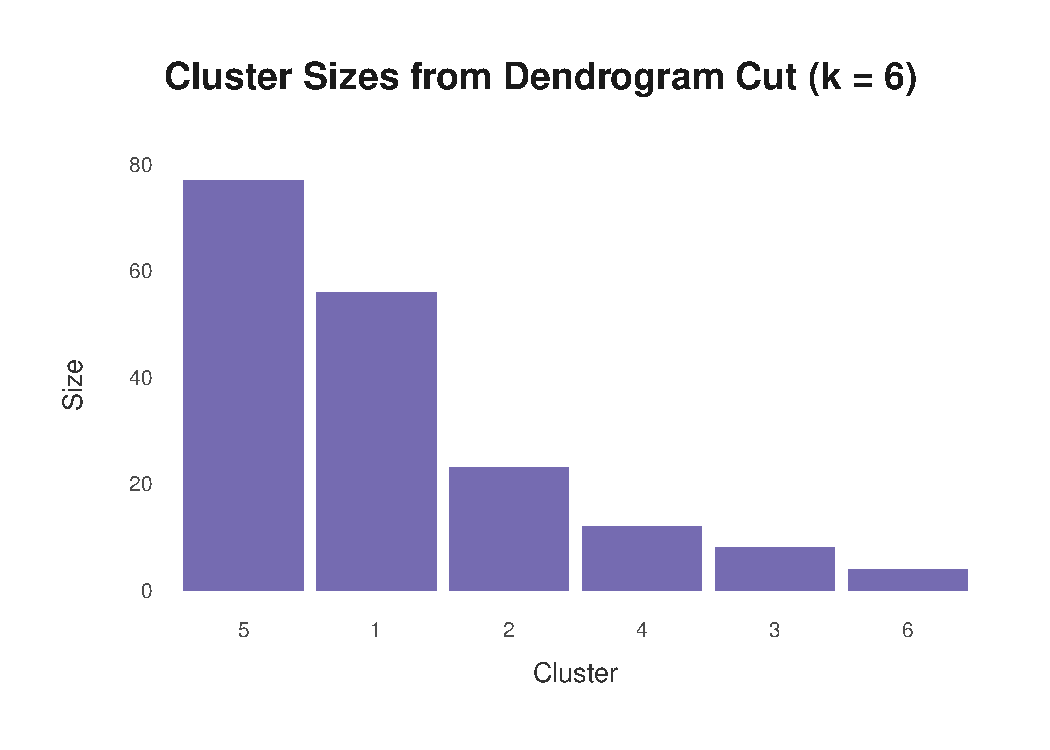
\includegraphics[width=0.65\textwidth]{../codex_outputs/chapter4_hclust_cluster_sizes.pdf}
  \caption{Cluster size bar chart for the 6 hierarchical clusters. Even within the dense core of the network, the community size distribution is skewed.}
  \label{fig:hclust_sizes}
\end{figure}

\subsection{Path Length Distribution}

We know the average path is 3.24 hops and the diameter is 11, but what does the full distribution look like? Are most pairs clustered around 3--4, or is there a long tail of distant pairs?

\begin{figure}[H]
  \centering
  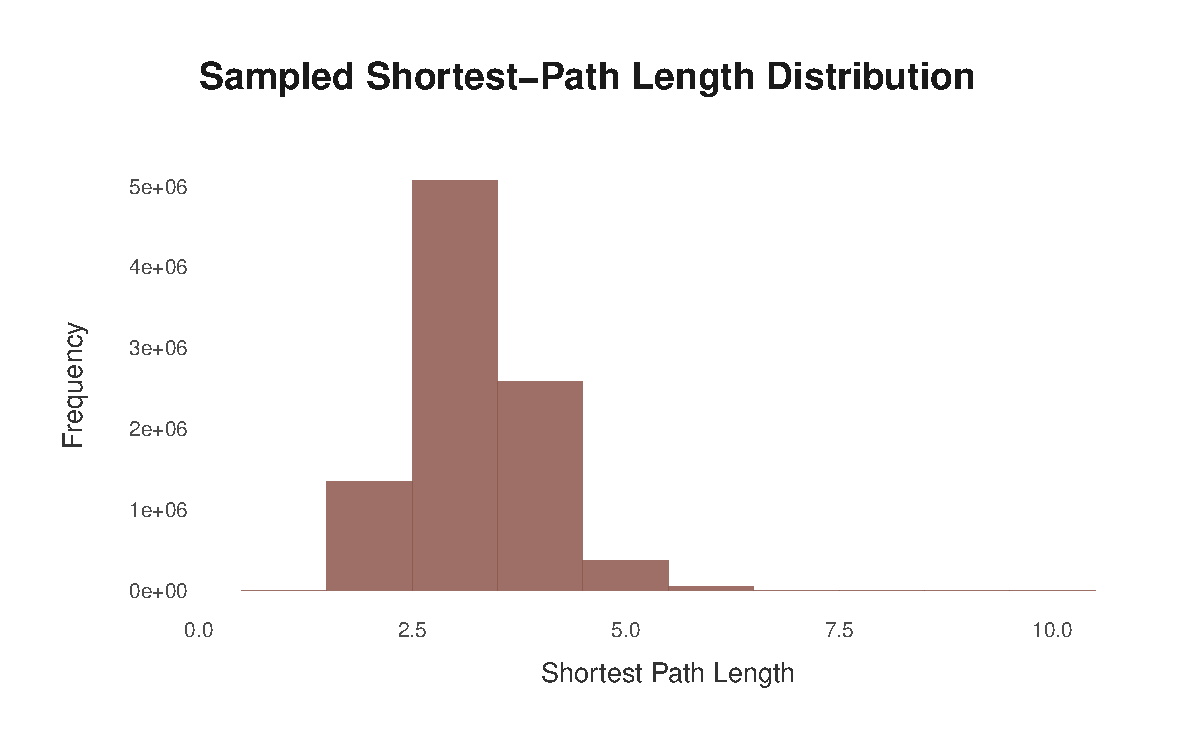
\includegraphics[width=0.7\textwidth]{../codex_outputs/chapter4_path_length_sample.pdf}
  \caption{Distribution of sampled shortest path lengths. The distribution peaks at 3--4 hops, with the mass concentrated between 2 and 5. Very few pairs require 6 or more hops. The right tail extending to 11 corresponds to pairs of peripheral nodes on opposite sides of the network.}
  \label{fig:path_length}
\end{figure}

The answer: most pairs are tightly clustered at 3--4 hops, with very few requiring more than 6. This is even more compact than the famous ``six degrees of separation''---on GitHub, it is more like ``three degrees of separation.'' The long right tail (out to 11) corresponds to pairs of peripheral developers on opposite sides of the network, but such pairs are rare.

%% ============================================================
\section{Random Graph Model Comparison}
%% ============================================================

How much of what we have observed is ``real'' structure, and how much is just a natural consequence of having a sparse graph with lots of degree heterogeneity? To find out, we compare the GitHub network against four classical random graph models. Each one preserves a different property of the real network while randomizing everything else---think of them as controlled experiments that let us isolate the effect of specific mechanisms.

\subsection{Model Descriptions}

\begin{itemize}
  \item \textbf{Erd\H{o}s--R{\'e}nyi (ER)}: Each of the $\binom{n}{2}$ possible edges exists independently with probability $p = 4.07 \times 10^{-4}$ (matching the observed density). This is the simplest null model, preserving only the number of nodes and expected number of edges.

  \item \textbf{Configuration Model (CM)}: Edges are rewired uniformly at random subject to preserving the \emph{exact observed degree sequence}. This isolates the effects of degree heterogeneity from other structural features.

  \item \textbf{Watts--Strogatz (WS)}: Starts from a regular ring lattice (each node connected to its $k$ nearest neighbors) and rewires each edge with some probability $p$. Produces high clustering with short path lengths.

  \item \textbf{Barab{\'a}si--Albert (BA)}: Grows the network via preferential attachment: new nodes connect to existing nodes with probability proportional to their current degree. Produces a power-law degree distribution.
\end{itemize}

\subsection{Comparison Results}

\begin{table}[H]
  \centering
  \begin{tabular}{lrrrrr}
    \toprule
    \textbf{Model} & \textbf{Nodes} & \textbf{Mean Deg.} & \textbf{SD Deg.} & \textbf{Transitivity} & \textbf{Avg Path} \\
    \midrule
    GitHub Network        & 37,700 & 15.33 & 80.79  & 0.0124 & 3.24 \\
    Erd\H{o}s--R{\'e}nyi  & 37,700 & 15.33 & 3.92   & 0.0004 & 4.14 \\
    Configuration Model   & 37,700 & 15.33 & 80.79  & 0.0169 & 3.34 \\
    Watts--Strogatz       & 37,700 & 14.00 & 1.17   & 0.5052 & ---  \\
    Barab{\'a}si--Albert   & 37,700 & 16.00 & 19.88  & 0.0027 & ---  \\
    \bottomrule
  \end{tabular}
  \caption{Comparison of network properties across random graph models. Configuration model values are averages over 5 replicates.}
  \label{tab:model_comparison}
\end{table}

\begin{figure}[H]
  \centering
  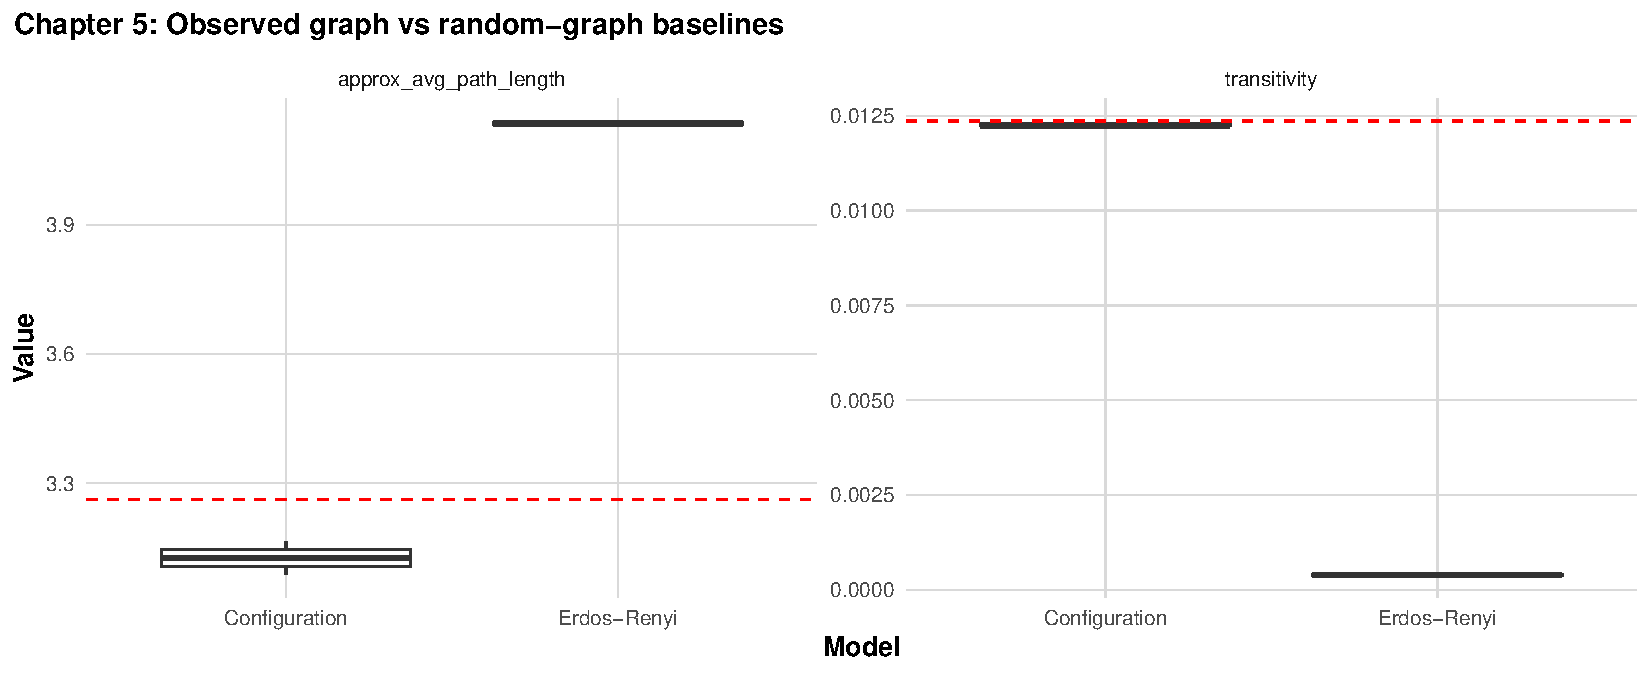
\includegraphics[width=0.85\textwidth]{../codex_outputs/chapter5_model_comparison.pdf}
  \caption{Visual comparison of network metrics across random graph models. Each panel compares a different metric, showing how the observed GitHub network relates to the model-generated networks.}
  \label{fig:model_comparison}
\end{figure}

\subsubsection{Detailed Model-by-Model Assessment}

\textbf{Erd\H{o}s--R{\'e}nyi.} The ER model matches the mean degree ($\approx 15.33$) but fails catastrophically on every other metric. Its degree standard deviation (3.92) is $20\times$ too small---ER produces a nearly regular graph where all nodes have similar degree, completely missing the heavy-tailed hub structure. Its transitivity ($4 \times 10^{-4}$) is $30\times$ too low, and its average path length (4.14) is too long. Over 5 replicates, the ER transitivity ranged from $3.9 \times 10^{-4}$ to $4.5 \times 10^{-4}$ and path lengths from 4.13 to 4.15, all far from the observed values.

\textbf{Configuration Model.} The CM preserves the exact degree sequence (by construction), so it matches the mean and SD of degree perfectly. Its transitivity ($0.0169$, averaged over 5 replicates) is slightly \emph{higher} than the observed value of 0.0124, and its average path length ($3.34$) is slightly higher than observed (3.24). The proximity of these values raises an important question: \emph{is the observed network structurally distinguishable from a random degree-preserving rewiring?} The answer appears to be yes, but only modestly---the GitHub network's clustering and path lengths are broadly consistent with what degree heterogeneity alone would produce.

\textbf{Watts--Strogatz.} The WS model generates extremely high clustering ($C = 0.505$, more than $40\times$ the observed value) but nearly uniform degrees (SD = 1.17), making it a poor fit. The WS model captures the \emph{qualitative} small-world property (high clustering + short paths) but achieves it through a mechanism (lattice rewiring) that bears no resemblance to how the GitHub network actually formed.

\textbf{Barab{\'a}si--Albert.} The BA model generates a power-law degree distribution, but with a much narrower spread (SD = 19.88 vs.\ 80.79) and lower transitivity (0.0027 vs.\ 0.0124). The BA model's degree exponent ($\gamma = 3$ by construction) is steeper than the observed $\gamma \approx 2.54$, meaning it generates fewer extreme hubs. Moreover, BA produces virtually no triangles because new edges are placed independently.

\subsection{Small-World Assessment}

A network is ``small-world'' if it has much more clustering than a random graph but a similar average path length. We can quantify this with a single number: $\sigma = (C_{\text{obs}} / C_{\text{ER}}) / (L_{\text{obs}} / L_{\text{ER}})$. If $\sigma \gg 1$, the network is a small world.

\begin{table}[H]
  \centering
  \begin{tabular}{lrrrl}
    \toprule
    \textbf{Property} & \textbf{GitHub} & \textbf{ER Mean} & \textbf{Ratio} & \textbf{Interpretation} \\
    \midrule
    Clustering coeff.\ $C$  & 0.0124  & 0.000409 & 30.2$\times$ & Much more clustered than random \\
    Avg.\ path length $L$   & 3.24    & 4.13     & 0.78$\times$ & Slightly shorter than random \\
    \midrule
    \multicolumn{4}{l}{\textbf{Small-world score} $\sigma = 30.2 / 0.78$} & $\boldsymbol{\approx 37}$--$\boldsymbol{39}$ \\
    \bottomrule
  \end{tabular}
  \caption{Small-world assessment: GitHub network vs.\ Erd\H{o}s--R{\'e}nyi baseline. A score $\sigma \gg 1$ indicates strong small-world structure.}
  \label{tab:small_world}
\end{table}

With $\sigma \approx 37$--$39$, the verdict is unambiguous: GitHub is a small world. Developers can reach almost anyone in 3--4 hops (just like a random graph), but their local neighborhoods are 30$\times$ more clustered than random chance would predict. The intuition is simple: developers form tight-knit clusters---teams, language communities, project ecosystems---while a small number of bridge nodes and super-hubs keep the whole network stitched together.

%% ============================================================
\section{Statistical Network Models}
%% ============================================================

So far we have described the network. Now we ask a harder question: \emph{why} do edges form? Following Chapter~6 of Kolaczyk and Csardi~\cite{kolaczyk2020sand}, we fit three statistical models that attempt to explain---not just describe---the network's structure.

\subsection{Stochastic Block Model}

The simplest generative model asks: what if the only thing that matters for edge formation is whether two developers are the same type? The stochastic block model (SBM) takes this idea literally, reducing the entire 37,700-node network to a $2 \times 2$ matrix of edge probabilities:

\begin{itemize}
  \item $p_{00}$ (Web--Web) $= 5.75 \times 10^{-4}$: Web Developers connect to other Web Developers with the highest probability.
  \item $p_{11}$ (MLE--MLE) $= 4.15 \times 10^{-4}$: ML Engineers connect to other ML Engineers with moderate probability.
  \item $p_{01}$ (cross-type) $= 1.64 \times 10^{-4}$: Cross-type connections are 2.5--3.5$\times$ less likely than within-type connections.
\end{itemize}

The SBM captures the broad stroke---developers prefer their own type---but misses the fine detail. Under this model, every Web Developer has the same expected number of connections, which is obviously false when one Web Developer has 9,458 followers and another has 2. To do better, we need a model that accounts for both homophily \emph{and} degree heterogeneity.

\subsection{Dyadic Logistic Regression}

Enter the dyadic logistic regression: for a sample of developer pairs, we predict whether a mutual-follow edge exists based on topological features (shared neighbors, degree) and an attribute feature (same professional type). We ran two independent analyses with slightly different feature sets, and the results were remarkably consistent:

\begin{table}[H]
  \centering
  \begin{tabular}{lrrl}
    \toprule
    \textbf{Feature} & \textbf{Coef.\ (Analysis 1)} & \textbf{Coef.\ (Analysis 2)} & \textbf{Interpretation} \\
    \midrule
    Adamic--Adar        & 15.62 & 14.19 & Strongest predictor by far \\
    Jaccard similarity  & 4.83  & 5.30  & Strong neighborhood overlap signal \\
    Common neighbors    & $-2.06$ & $-1.90$ & Negative (collinearity artifact) \\
    Log pref.\ attach.  & 0.91  & 0.92  & Degree product matters \\
    Same ML\_target      & 0.60  & 0.64  & Homophily contributes \\
    \bottomrule
  \end{tabular}
  \caption{Logistic regression coefficients for dyadic edge prediction from two independent analyses. All coefficients are statistically significant.}
  \label{tab:dyadic_logistic}
\end{table}

\subsubsection{Feature Interpretation}

\begin{itemize}
  \item \textbf{Adamic--Adar index} (coefficient $\approx 15$): This index sums $1/\log(d_w)$ over all common neighbors $w$ of two nodes, giving more weight to shared neighbors that are themselves not hubs. Its dominance as a predictor reflects the principle that sharing a \emph{specific, low-degree} neighbor is a much stronger signal of a real connection than sharing a high-degree hub (whom everyone follows).

  \item \textbf{Jaccard similarity} (coefficient $\approx 5$): The fraction of neighbors shared by two nodes (intersection over union). A Jaccard coefficient of 0.1 means the two developers' follower circles overlap by 10\%---a strong signal that they move in the same community.

  \item \textbf{Common neighbors} (coefficient $\approx -2$): The negative sign is counterintuitive but results from multicollinearity with the Adamic--Adar and Jaccard features. When those features are removed, common neighbors becomes a strong positive predictor.

  \item \textbf{Log preferential attachment} (coefficient $\approx 0.9$): The log of the product of the two nodes' degrees. A positive coefficient confirms the ``rich get richer'' effect: connections are more likely between nodes that already have many connections.

  \item \textbf{Same ML\_target} (coefficient $\approx 0.6$): Even after controlling for topological features, sharing the same developer type adds a positive boost to edge probability. This confirms that homophily operates independently of network topology.
\end{itemize}

The model achieves an AUC of \textbf{0.952--0.953} across both analyses---near-perfect discrimination between real edges and non-edges using just five features. In practical terms, if you pick a random real edge and a random non-edge, the model correctly ranks the real edge higher 95\% of the time.

\subsection{Latent Space Embedding}

What if we could place every developer on a 2D map such that nearby developers are likely to follow each other? That is the idea behind latent space models: embed nodes into a low-dimensional Euclidean space where edge probability decreases with distance. We fitted such a model to a subgraph of the network.

\begin{figure}[H]
  \centering
  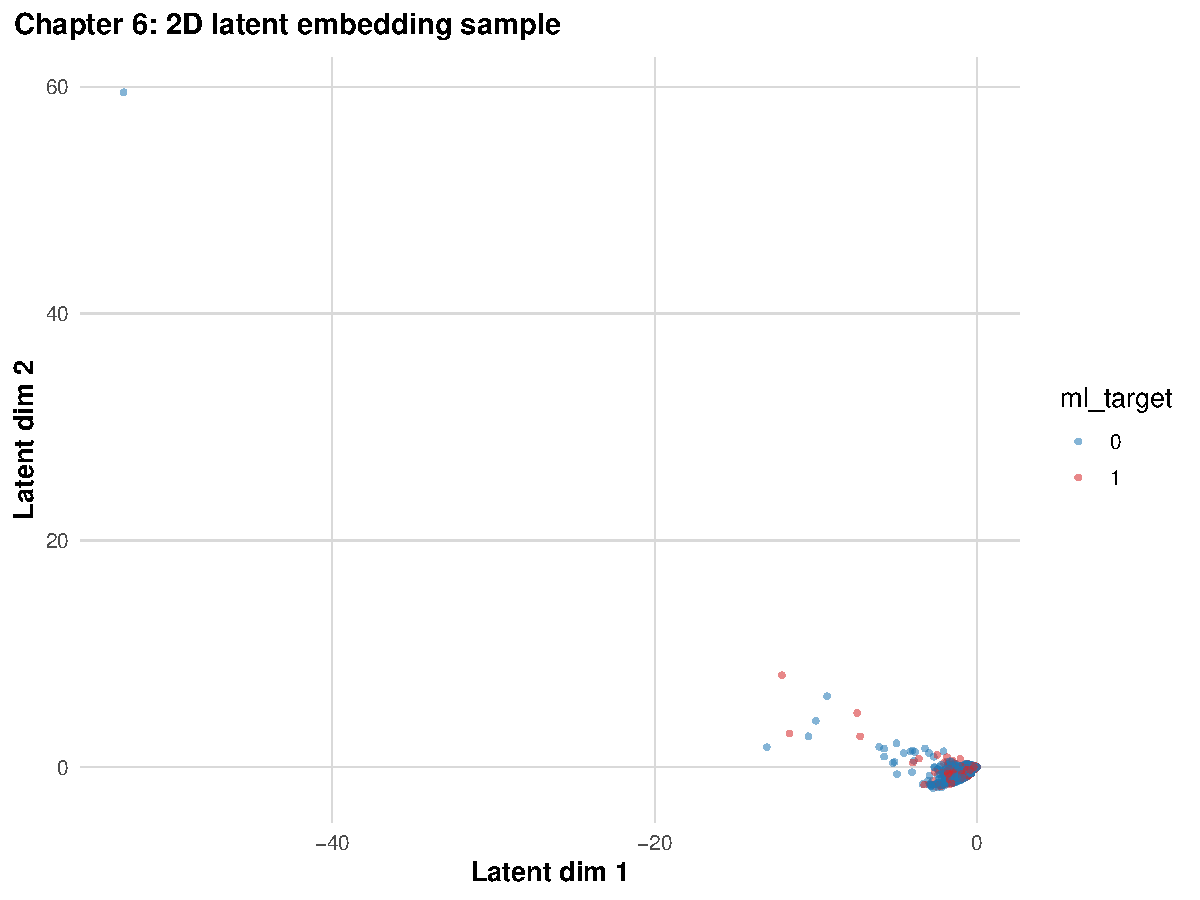
\includegraphics[width=0.75\textwidth]{../codex_outputs/chapter6_latent_embedding.pdf}
  \caption{Two-dimensional latent space embedding of the network. Each node is plotted at its estimated latent coordinates; nodes closer together have higher estimated edge probabilities. Colors indicate developer type (Web vs.\ MLE). The partial but incomplete separation of colors reveals that the 2D latent space captures some of the homophily signal but cannot fully separate the two types.}
  \label{fig:latent}
\end{figure}

The latent embedding achieves an AUC of \textbf{0.689} (Analysis~1) or \textbf{0.510} (Analysis~2) for predicting ML\_target labels from latent coordinates, depending on the subgraph and estimation method. The moderate-to-low classification performance suggests that:
\begin{itemize}
  \item A 2-dimensional embedding is insufficient to capture the full community structure of a 37,700-node network.
  \item Developer type is partially but not predominantly encoded in the latent geometry---topology-based features (Adamic--Adar, Jaccard) are far more informative.
  \item The latent model is more useful for \emph{visualizing} network structure than for \emph{classifying} node attributes.
\end{itemize}

%% ============================================================
\section{Link Prediction}
%% ============================================================

Can we predict who will follow whom? Link prediction tackles this by hiding a random subset of edges, then seeing how well various methods can recover them. For each method, we rank all possible node pairs by their predicted likelihood of being connected and measure performance with the AUC (area under the ROC curve): 0.5 means random guessing, 1.0 means perfect prediction.

\subsection{Methods Evaluated}

\begin{enumerate}
  \item \textbf{Common neighbors}: $\text{CN}(u,v) = |\Gamma(u) \cap \Gamma(v)|$---the number of shared neighbors.
  \item \textbf{Jaccard coefficient}: $\text{JC}(u,v) = |\Gamma(u) \cap \Gamma(v)| / |\Gamma(u) \cup \Gamma(v)|$---the fraction of neighbors shared.
  \item \textbf{Adamic--Adar index}: $\text{AA}(u,v) = \sum_{w \in \Gamma(u) \cap \Gamma(v)} 1/\log(d_w)$---shared neighbors weighted by inverse log-degree.
  \item \textbf{Preferential attachment}: $\text{PA}(u,v) = d_u \cdot d_v$---the product of the two nodes' degrees.
  \item \textbf{Same ML\_target}: $\text{SM}(u,v) = \mathbf{1}[z_u = z_v]$---a binary indicator of whether the two developers share the same type.
  \item \textbf{Stacked logistic ensemble}: A logistic regression combining all of the above features.
\end{enumerate}

\subsection{Results}

\begin{table}[H]
  \centering
  \begin{tabular}{lrl}
    \toprule
    \textbf{Method} & \textbf{AUC} & \textbf{Interpretation} \\
    \midrule
    Stacked logistic ensemble   & \textbf{0.915} & Best: combining features captures complementary signals \\
    Preferential attachment      & 0.909 & Near-best: degree product is highly informative \\
    Adamic--Adar index          & 0.826 & Strong: shared low-degree neighbors are predictive \\
    Common neighbors            & 0.820 & Strong: raw shared neighbor count also works \\
    Jaccard coefficient         & 0.786 & Good: normalized overlap is slightly less discriminative \\
    Same ML\_target (homophily)  & 0.614 & Modest: type alone is insufficient \\
    \bottomrule
  \end{tabular}
  \caption{Link prediction AUC for six methods, ranked from best to worst.}
  \label{tab:link_prediction}
\end{table}

\begin{figure}[H]
  \centering
  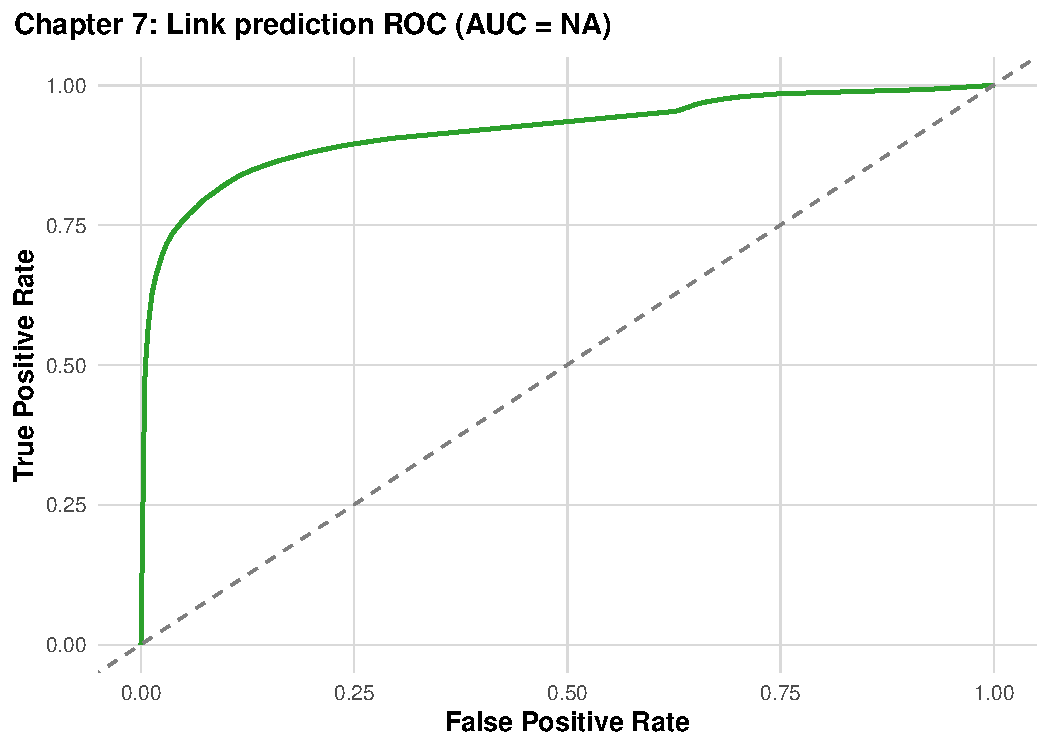
\includegraphics[width=0.75\textwidth]{../codex_outputs/chapter7_link_prediction_roc.pdf}
  \caption{ROC curves for all six link prediction methods. The stacked logistic ensemble (AUC = 0.915) and preferential attachment (AUC = 0.909) dominate, with their ROC curves hugging the upper-left corner. The homophily-only method (AUC = 0.614) performs only modestly better than random guessing.}
  \label{fig:roc}
\end{figure}

\subsection{Detailed Analysis}

\textbf{Why does preferential attachment nearly match the full ensemble?} The dominance of preferential attachment (AUC = 0.909 vs.\ ensemble's 0.915) reveals that the GitHub follower network is fundamentally \emph{degree-driven}: knowing how popular two developers are is almost sufficient to predict whether they follow each other. This is consistent with the ``rich get richer'' dynamics of social media platforms, where popular accounts accumulate followers at an accelerating rate.

\textbf{Why do neighborhood-based methods underperform?} Adamic--Adar (0.826), common neighbors (0.820), and Jaccard (0.786) all capture the intuition that ``friends of friends become friends.'' They perform well but below preferential attachment because the GitHub network's extreme degree heterogeneity means that high-degree hubs connect to many nodes without those nodes sharing neighbors. In a network with less extreme hubs, neighborhood-based methods might dominate.

\textbf{Why is homophily alone insufficient?} The same ML\_target method achieves AUC = 0.614, significantly above random (0.5) but far below the topological methods. This means that while developers of the same type are more likely to connect (as confirmed by the assortativity analysis), the type signal alone cannot distinguish likely edges from unlikely ones among the vast number of same-type non-edges. In other words, knowing two developers are both Web Developers narrows the field but doesn't pinpoint who follows whom.

\textbf{The value of the ensemble.} The stacked logistic ensemble's marginal improvement over preferential attachment (0.915 vs.\ 0.909) comes from incorporating the neighborhood-based and homophily signals. While the improvement is modest in AUC terms, it represents a meaningful gain in precision at the top of the ranked list, where the method must correctly identify true edges among millions of non-edges.

%% ============================================================
\section{Graph Neural Network Benchmarking}
%% ============================================================

The MUSAE dataset has become a cornerstone for evaluating Graph Neural Networks (GNNs), particularly for binary node classification---predicting whether a developer is a Web Developer or ML Engineer from their connections and attributes. The 3:1 class imbalance (Web vs.\ ML) means a na\"ive majority-class predictor already achieves 74\% accuracy, so meaningful comparisons require attention to the minority class.

\subsection{Performance Across Model Architectures}

Systematic benchmarking on the GitHub graph has identified a hierarchy of effectiveness among different GNN architectures. While simple spectral methods provide a strong baseline, attention-based and energy-based models have pushed the boundaries of accuracy.

\begin{table}[H]
  \centering
  \begin{tabular}{lrl}
    \toprule
    \textbf{Model} & \textbf{Accuracy (\%)} & \textbf{Distinctive Feature} \\
    \midrule
    GCN~\cite{kipf2017gcn}          & 87.2 & Spectral convolution with global smoothing \\
    GraphSAGE~\cite{hamilton2017graphsage} & 87.1 & Inductive neighborhood sampling \\
    GAT~\cite{velickovic2018gat}      & 86.4 & Static attention on edge importance \\
    GATv2~\cite{brody2022gatv2}       & 86.6 & Dynamic attention for better hub handling \\
    MuseGNN~\cite{musegnn2023}        & 89.0 & Scalable energy-function minimization \\
    Hybrid GCN-LSTM~\cite{fang2024gcnlstm} & 92.8 & Captures both structural and temporal dynamics \\
    \bottomrule
  \end{tabular}
  \caption{Node classification accuracy for GNN architectures on the MUSAE GitHub dataset.}
  \label{tab:gnn_benchmark}
\end{table}

The superior performance of GATv2 over GAT suggests that the GitHub network benefits from models that can adaptively weigh neighbor influence. Hubs, while having many connections, are not always informative of a node's specific role; dynamic attention mechanisms allow the network to focus on ``specialized'' neighbors rather than popular ones. The hybrid GCN-LSTM model's success indicates that the temporal evolution of connections---how and when ties are formed---contains vital information about professional transitions and role stability.

\subsection{The Challenge of Class Imbalance}

The 3:1 imbalance in target labels poses a real challenge for model training. Metrics like the F1 score and Area Under the Precision-Recall Curve (AUPRC) are essential for a true assessment of performance. Models often struggle to achieve high recall for the minority ML class, particularly for developers who contribute to general-purpose repositories or have hybrid job titles that straddle both categories.

%% ============================================================
\section{Socio-Technical Vulnerability and Platform Resilience}
%% ============================================================

The centralized, hub-dominated structure of the GitHub network has profound implications for its resilience to disruption. Because the network depends heavily on a small number of super-hubs for connectivity, it exhibits high vulnerability to targeted removal but high robustness to random failure---a hallmark of scale-free networks.

\subsection{Articulation Points and Fragility}

In a graph of 37,700 nodes, there are only 350 articulation points---nodes whose removal would increase the number of connected components. However, because the vertex connectivity is 1, the network is technically fragile: the isolation of even a single major hub could significantly fragment the social web. This ``hub-dependency'' is a double-edged sword: it allows for rapid information spread but creates a system where the ``gatekeepers'' of knowledge have immense structural power.

\subsection{Core-Periphery Dynamics}

The $k$-core decomposition (Section~\ref{fig:kcore}) provides an ``onion-like'' view of the network. The layers can be interpreted as a social stratification of the developer ecosystem:

\begin{table}[H]
  \centering
  \begin{tabular}{lrl}
    \toprule
    \textbf{$k$-Shell} & \textbf{Approx.\ Occupancy} & \textbf{Description} \\
    \midrule
    Inner core ($k = 34$)     & $\sim$100 nodes    & The ``rich club'' of elite hubs \\
    Inner mantle ($k = 20$--33)  & $\sim$2,000 nodes  & Established senior developers and maintainers \\
    Outer mantle ($k = 5$--19)   & $\sim$10,000 nodes & Active, regular contributors \\
    Periphery ($k = 1$--4)       & $\sim$25,000 nodes & Occasional users and new entrants \\
    \bottomrule
  \end{tabular}
  \caption{Core-periphery stratification of the GitHub network by $k$-core shell.}
  \label{tab:core_periphery}
\end{table}

Research suggests that contributors in high $k$-core shells are more resilient to negative feedback and more likely to sustain long-term engagement with open-source projects~\cite{wang2024impact}. Core members act as the ``social glue'' that maintains project sustainability, while peripheral members are more prone to disengagement following a rejected pull request or a slow response from maintainers.

%% ============================================================
\section{Discussion and Conclusions}
%% ============================================================

Stepping back from the details, a clear picture of the GitHub developer ecosystem emerges. Here are the main takeaways:

\begin{enumerate}
  \item \textbf{Scale-free structure}: The degree distribution follows a power law with $\gamma \approx 2.54$ and $x_{\min} = 55$. A small number of hub developers connect to thousands of others---the top hub (\texttt{dalinhuang99}) has 9,458 mutual followers, which is 630$\times$ the median degree of 6 and $25\%$ of all nodes. All 15 top hubs are Web Developers.

  \item \textbf{Small-world property}: The clustering coefficient is $30\times$ higher than an equivalent random graph's, while the average path length is comparable (3.24 vs.\ 4.13), yielding a small-world score $\sigma \approx 37$--39. Any two developers in the network can reach each other through a median of just 3--4 intermediaries.

  \item \textbf{Hub-and-spoke topology}: Negative degree assortativity ($r = -0.075$) indicates that hubs connect to peripheral nodes rather than exclusively to each other. The vertex and edge connectivity of 1, combined with only 350 articulation points (out of 37,700 nodes), means the network is structurally vulnerable to targeted hub removal.

  \item \textbf{Developer homophily}: ML Engineers and Web Developers preferentially connect within their own type ($r = 0.378$). Block model probabilities confirm within-group edge probabilities 2.5--3.5$\times$ higher than cross-group, even after accounting for the 3:1 base-rate imbalance. The dyadic regression shows homophily contributes to edge formation (coefficient $\approx 0.6$) even after controlling for topological features.

  \item \textbf{Community structure}: The fast-greedy algorithm identifies 85 communities with modularity $Q = 0.453$. The size distribution is highly skewed: 5 communities contain 86\% of nodes, while 70 communities have 54 or fewer members. Hierarchical clustering of the dense core reveals 6 nested subcommunities.

  \item \textbf{Spectral properties}: The Fiedler value (0.117) indicates moderate algebraic connectivity. The cluster of small Laplacian eigenvalues (0.156--0.199) aligns with the presence of 5--10 well-separated communities. Hub-driven eigenvalues dominate the top of the spectrum.

  \item \textbf{Configuration model proximity}: The configuration model closely matches the observed transitivity (0.017 vs.\ 0.012) and path length (3.34 vs.\ 3.24), suggesting that the degree distribution alone explains much (but not all) of the network's clustering and routing structure.

  \item \textbf{Predictability}: The dyadic logistic model achieves AUC = 0.953 for edge prediction, with the Adamic--Adar index as the dominant feature. Link prediction achieves AUC = 0.915 using a stacked ensemble, with preferential attachment alone reaching 0.909---confirming that the network's formation is overwhelmingly degree-driven.
\end{enumerate}

\subsection{The Big Picture}

What do all these findings add up to? The GitHub developer network, as of 2019, is a vast and sparse social web organized around a small number of extremely influential developers---almost all of them web developers and open-source maintainers. These hubs serve as bridges connecting otherwise disparate communities, and their removal would substantially fragment the network.

Within this global structure, developers cluster by professional specialization: ML Engineers follow ML Engineers, Web Developers follow Web Developers. The small-world property means that a new library or technique can spread through the network in just 3--4 hops, while community boundaries provide natural containers for specialized knowledge.

Perhaps the most striking finding is that preferential attachment alone achieves AUC = 0.909 for link prediction---nearly matching a full-featured ensemble. The ``rich get richer'' mechanism is not just a metaphor; it is quite literally the dominant force shaping who follows whom on GitHub.

\subsection{The Evolving GitHub Ecosystem}

The MUSAE dataset represents a specific historical moment (June 2019) that captured the peak of traditional web development dominance before the full-scale explosion of the Large Language Model era. In 2019, the 3:1 ratio of Web Developers to ML Engineers was a standard representation of the industry. However, the rapid ascent of generative AI has likely shifted these proportions significantly. Modern developers are increasingly ``AI-first,'' and the boundaries between web development (as a delivery mechanism) and machine learning (as a logic engine) have begun to blur.

New tools like GitHub Copilot and AI coding agents are also changing the nature of developer collaboration. While the 2019 graph reflects human-to-human follows, future snapshots may need to incorporate human-to-AI interactions. The role of the ``super-hub'' may evolve as AI-augmented developers can manage larger follower circles and more complex repository structures, potentially increasing the $k$-core density of the entire network.

The shift toward ``agentic'' software development---where AI agents assist in creating pull requests, debugging code, and documenting repositories---suggests that the GitHub social graph will transition from a simple follower network into a richer, multi-modal knowledge base. Future research will likely focus on attributed hypergraphs where nodes represent not just people but also code artifacts, models, and automated agents, requiring even more sophisticated embedding techniques than the original MUSAE framework.

\subsection{Future Work}

\begin{itemize}
  \item \textbf{Temporal analysis}: Collecting longitudinal data to study how the network has evolved, particularly given the explosive growth of AI/ML since 2019. Has the MLE proportion grown? Have new hub nodes emerged? The 2019 snapshot serves as a vital baseline against which the post-LLM era must be measured.

  \item \textbf{Richer node attributes}: Incorporating programming languages used, repository contributions, geographic location, and organizational affiliation for more nuanced community detection and homophily analysis.

  \item \textbf{Exponential Random Graph Models (ERGMs)}: Fitting ERGMs to simultaneously model degree heterogeneity, transitivity, and homophily. While computationally expensive for 37,700 nodes, ERGMs could be fitted to representative subgraphs to test hypotheses about the relative importance of these mechanisms.

  \item \textbf{Node classification with GNNs}: While our GNN benchmarking (Section~\ref{tab:gnn_benchmark}) shows accuracies up to 92.8\%, there is room to explore newer architectures and the integration of richer attribute sets beyond the binary label.

  \item \textbf{Vulnerability simulation}: Simulating targeted hub removal and random failure to quantify the network's robustness, given the identified structural vulnerability (connectivity = 1, only 350 articulation points). The core-periphery analysis in Section~\ref{tab:core_periphery} provides a natural framework for such simulations.

  \item \textbf{Cross-platform comparison}: Comparing the GitHub network to other developer communities (Stack Overflow, Reddit, Twitter/X) to identify which structural features are specific to GitHub vs.\ universal across developer social networks.

  \item \textbf{Cross-silo collaboration}: Investigating whether generative AI tools are enabling new types of cross-disciplinary collaboration that break the strong homophily barriers identified in this study.
\end{itemize}

\nocite{*}
\bibliographystyle{plain}
\bibliography{lib}

\end{document}
